% ============================================
% AEGIS Entropy --- Final Report (Combined)
% Adaptive Entropy-based Gateway for Intrusion Suppression
% Single-file version — all chapters inlined
% ============================================
\documentclass[12pt,a4paper]{report}

% --- Encoding & Language ---
\usepackage[utf8]{inputenc}
\usepackage[T1]{fontenc}
\usepackage[english]{babel}
\usepackage{lmodern}

% --- Page Layout ---
\usepackage[left=2.5cm,right=2.5cm,top=2.5cm,bottom=2.5cm]{geometry}
\setlength{\parindent}{0pt}
\setlength{\parskip}{0.65em}
\renewcommand{\arraystretch}{1.25}

% --- Math ---
\usepackage{amsmath,amssymb}

% --- Graphics ---
\usepackage{graphicx}
\graphicspath{
    {figures/data/}
    {figures/capture/}
}
\usepackage{float}
\usepackage{caption}
\usepackage{subcaption}

% --- Tables ---
\usepackage{array}
\usepackage{longtable}
\usepackage{booktabs}
\usepackage{tabularx}
\usepackage[table]{xcolor}

% --- Lists ---
\usepackage{enumitem}
\setlist[itemize]{topsep=0.2em,itemsep=0.2em}
\setlist[enumerate]{topsep=0.2em,itemsep=0.25em}

% --- Code Listings ---
\usepackage{listings}
\lstdefinestyle{pythonstyle}{
    language=Python,
    basicstyle=\ttfamily\small,
    keywordstyle=\color{blue}\bfseries,
    stringstyle=\color{red},
    commentstyle=\color{gray}\itshape,
    numbers=left,
    numberstyle=\tiny\color{gray},
    stepnumber=1,
    numbersep=5pt,
    backgroundcolor=\color{gray!5},
    frame=single,
    rulecolor=\color{gray!30},
    breaklines=true,
    showstringspaces=false,
    tabsize=4,
    captionpos=b
}
\lstset{style=pythonstyle}

% --- TikZ ---
\usepackage{tikz}
\usetikzlibrary{shapes.geometric, arrows.meta, positioning, calc, decorations.pathmorphing, fit, backgrounds}
\usepackage{pgfplots}
\pgfplotsset{compat=1.18}

% --- Colors for diagrams ---
\definecolor{darkbg}{HTML}{0b0f19}
\definecolor{cyan}{HTML}{22d3ee}
\definecolor{green}{HTML}{34d399}
\definecolor{red}{HTML}{f87171}
\definecolor{amber}{HTML}{fbbf24}
\definecolor{purple}{HTML}{a78bfa}
\definecolor{codebg}{HTML}{1a2332}
\definecolor{codegray}{HTML}{94a3b8}
\definecolor{LightGray}{HTML}{F2F2F2}
\definecolor{LightBlue}{HTML}{D9EAF7}

% --- Hyperlinks ---
\usepackage{hyperref}
\hypersetup{
    colorlinks=true,
    linkcolor=blue!70!black,
    urlcolor=blue!60!black,
    citecolor=blue!70!black,
    pdftitle={AEGIS Entropy --- Final Report},
    pdfauthor={AEGIS Entropy Team}
}

% --- Headers & Footers ---
\usepackage{fancyhdr}
\pagestyle{fancy}
\fancyhf{}
\fancyhead[L]{\small\textsc{AEGIS Entropy}}
\fancyhead[R]{\small\textsc{Final Report}}
\fancyfoot[C]{\thepage}
\renewcommand{\headrulewidth}{0.4pt}

% --- Chapter/Section Formatting ---
\usepackage{titlesec}
\titleformat{\chapter}[display]
    {\normalfont\Large\bfseries\color{blue!80!black}}
    {\chaptertitlename\ \thechapter}
    {0.5em}
    {}
\titleformat{\section}{\normalfont\large\bfseries\color{blue!70!black}}{\thesection}{1em}{}
\titleformat{\subsection}{\normalfont\normalsize\bfseries\color{blue!60!black}}{\thesubsection}{1em}{}

% --- Custom Commands ---
\newcolumntype{Y}{>{\raggedright\arraybackslash}X}
\newcolumntype{L}[1]{>{\raggedright\arraybackslash}p{#1}}
\newcommand{\code}[1]{\texttt{\detokenize{#1}}}

% --- Placeholder Command ---
\newcommand{\todo}[1]{\textcolor{red}{\textbf{[TODO: #1]}}}
\newcommand{\tobewritten}[1]{\textcolor{orange}{\textit{[To be written by #1]}}}

% ============================================
\begin{document}

% --- Title Page ---
\begin{titlepage}
\centering

% --- Logos at top corners ---
\begin{minipage}{0.45\textwidth}

\includegraphics[width=2.5cm]{logo-UIT.png}
\end{minipage}%
\hfill
\begin{minipage}{0.45\textwidth}
\raggedleft

\includegraphics[width=2.5cm]{ensa_logo.png}
\end{minipage}

\vspace{1cm}

% --- Institution ---
{\Large\textsc{Universit\'{e} Ibn Tofa\"{i}l --- K\'{e}nitra}}\\[0.3cm]
{\large\textsc{\'{E}cole Nationale des Sciences Appliqu\'{e}es de K\'{e}nitra}}\\[0.3cm]
{\normalsize\textsc{Fili\`{e}re : Ing\'{e}nierie des R\'{e}seaux et des Syst\`{e}mes de T\'{e}l\'{e}communication}}

\vspace{2cm}

\rule{\textwidth}{0.5pt}\\[0.8cm]

{\Huge\bfseries AEGIS}\\[0.4cm]
{\Large Machine Learning-Based Intrusion Detection\\and Active Defense System}

\vspace{0.8cm}
\rule{\textwidth}{0.5pt}

\vspace{2cm}

% --- Supervisor + Team ---
\begin{minipage}{0.85\textwidth}
\centering
\textbf{Encadr\'{e} par}\\[0.3cm]
Prof.\ Aniss Moumen\\[1cm]
\textbf{R\'{e}alis\'{e} par}\\[0.3cm]
\begin{tabular}{c}
Adil Lekhbioui \\
Khadija Nafia \\
El Yazid Hammoubel \\
Moulay Anas \\
El Kartouti Anas \\
\end{tabular}
\end{minipage}

\vfill

{\normalsize Ann\'{e}e universitaire 2025 -- 2026}
\end{titlepage}

% --- Table of Contents ---
\tableofcontents
\listoffigures
\listoftables
\newpage

% ============================================
% GENERAL INTRODUCTION
% ============================================
\section*{General Introduction}

The continuous digitalisation of organisations has turned network infrastructures into critical assets shared across LAN, cloud, wireless, and hybrid environments. Protecting these infrastructures is no longer limited to deploying firewalls or signature-based Intrusion Detection Systems; attackers now operate with adaptive, automated tools that probe networks for open services and vulnerabilities before launching targeted intrusions. Port scanning and network reconnaissance constitute the first phase of this kill chain, yet static rule-based defences struggle to keep pace with stealthy, low-rate, or previously unseen scanning strategies.

This situation raises a clear operational question: \textit{How can we detect and classify PortScan attacks from network traffic data (pcap/csv) in order to protect the infrastructure and alert SOC teams in real time?} Existing solutions either detect without responding or respond with manually maintained rules, leaving security teams overwhelmed by false positives and unable to counter reconnaissance before it escalates. There is therefore a need for an intelligent system that can learn behavioural patterns, classify suspicious activity, and enforce autonomous countermeasures.

AEGIS Entropy addresses this need by combining machine learning-driven detection with active deception. The system analyses network flow features with Random Forest, XGBoost, and Isolation Forest classifiers, and couples detections with Moving Target Defence and honeypot redirection to mislead and delay attackers. This report presents the complete design, implementation, and validation of AEGIS Entropy, beginning with the state of the art and progressing through data understanding, model training, capture environment, defence subsystem, integration, and final validation.
% ============================================
% Chapter 1: State of the Art
% ============================================

\chapter{State of the Art}\label{ch:state_of_art}

\section{Introduction}

Network intrusion detection has evolved from manually maintained signature databases to data-driven machine learning systems capable of recognising behavioural anomalies. This chapter reviews the foundations of port scan detection, compares the principal families of detection algorithms, and introduces the active defence concepts that underpin the AEGIS Entropy architecture. The objective is to position the project within the current research and industrial landscape, and to justify the technical choices made in the subsequent chapters.

The chapter is organised as follows. Section~\ref{sec:portscan} defines port scanning and presents a taxonomy of common techniques. Section~\ref{sec:ids} contrasts classical and AI-based intrusion detection approaches. Section~\ref{sec:ml_dl} compares Machine Learning and Deep Learning for intrusion detection and explains why Machine Learning was selected for this project. Section~\ref{sec:supervised_unsupervised} discusses supervised and unsupervised learning paradigms. Sections~\ref{sec:mtd} and~\ref{sec:honeypot} introduce Moving Target Defence and honeypot-based deception. Section~\ref{sec:soa_conclusion} concludes with the positioning of AEGIS Entropy.

\section{Port Scan Attack Detection}\label{sec:portscan}

\subsection{Definition}

Port scanning is the systematic probing of a host or network to identify open ports, active services, and potential vulnerabilities. It is almost always the first reconnaissance step of a cyberattack: before an adversary can exploit a service, they must know that the service exists and understand its behaviour. Port scans generate distinctive traffic patterns---half-open connections, high volumes of rejected packets, and unusual inter-arrival times---that can be distinguished from normal host-to-host communication when the right features are monitored.

From a machine learning perspective, port scan detection is a binary classification problem: given a set of flow-level or packet-level features, assign the label \textsc{Benign} or \textsc{PortScan}. The difficulty lies in the diversity of scanning strategies, the similarity of some scan patterns to legitimate behaviour, and the need to operate in real time.

\subsection{Taxonomy of Port Scan Techniques}

Table~\ref{tab:scan_taxonomy} summarises the most common port scan techniques. Each technique produces a different signature in terms of TCP flags, completion state, and response behaviour, which in turn determines the features most useful for detection.

\begin{table}[H]
\centering
\caption{Classification of port scan techniques}
\label{tab:scan_taxonomy}
\begin{tabularx}{\textwidth}{lX}
\toprule
\textbf{Scan Type} & \textbf{Description} \\
\midrule
SYN Scan & Half-open scan using SYN packets without completing the TCP handshake. Fast and stealthy because it avoids full connection logs. \\
TCP Connect & Full TCP connection establishment to each target port. Easier to detect but works without raw socket privileges. \\
UDP Scan & Sends UDP packets to detect open UDP services. Relies on ICMP "port unreachable" responses for closed ports. \\
XMAS Scan & Sets FIN, PSH, and URG flags to elicit responses from closed ports. Often blocked by modern stacks but still used for firewall mapping. \\
ACK Scan & Sends ACK packets to map firewall rules by analysing RST responses. Useful for determining whether a port is filtered. \\
Service Detection & Probes identified open ports for service version information after the initial scan. \\
OS Detection & Analyses TCP/IP stack behaviour to fingerprint the operating system of the target. \\
\bottomrule
\end{tabularx}
\end{table}

SYN scans and UDP scans are the most common in real-world reconnaissance, while XMAS and ACK scans are often used to evade simple stateless firewalls. Service and OS detection occur in later phases and produce longer, more structured sessions.

\section{Network Intrusion Detection Systems}\label{sec:ids}

\subsection{Signature-Based Detection}

Signature-based Intrusion Detection Systems (IDS) such as Snort and Suricata compare observed traffic against databases of known attack patterns. They are highly accurate when the attack signature is known and well-defined, and they provide clear, explainable alerts. However, they require continuous manual updates, cannot detect zero-day or polymorphic attacks, and often generate many alerts in environments with diverse legitimate traffic.

\subsection{Anomaly-Based Detection}

Anomaly-based IDS build a statistical or behavioural model of normal network activity and flag significant deviations. This approach can detect previously unseen attacks, including slow scans and custom reconnaissance tools. The main challenge is defining ``normal'' behaviour: legitimate administrative tools, vulnerability scanners, and cloud orchestration can all appear anomalous, leading to false positives.

\subsection{Classical IDS/IPS vs AI-Based IDS/IPS}

Artificial Intelligence, and more specifically machine learning, offers a fundamentally different approach. Rather than relying on manually curated rules, AI-based systems learn statistical models of normal and malicious behaviour from labelled traffic datasets such as CICIDS2017~\cite{cicids2017}. Table~\ref{tab:ids-comparison} contrasts the two paradigms.

\begin{table}[H]
\centering
\caption{Classical IDS/IPS vs.\ AI-Based IDS/IPS}
\label{tab:ids-comparison}
\begin{tabularx}{\textwidth}{XX}
\toprule
\textbf{Classical IDS/IPS} & \textbf{AI-Based IDS/IPS} \\
\midrule
Relies on predefined signatures & Learns behavioural patterns from data \\
Fails against unknown/novel attacks & Detects anomalies beyond known signatures \\
Requires constant manual updates & Self-adapts through model retraining \\
No autonomous response capability & Supports automated threat neutralisation \\
High false positive rate at scale & Optimised precision/recall via ML tuning \\
Static and network-topology-specific & Generalisable across diverse network types \\
\bottomrule
\end{tabularx}
\end{table}

AI-based detection is not a replacement for classical defences; it is a complementary layer that reduces alert fatigue and improves coverage against evolving reconnaissance techniques.

\section{Machine Learning vs Deep Learning for Intrusion Detection}\label{sec:ml_dl}

\subsection{Deep Learning Approaches}

Deep Learning approaches for intrusion detection include Convolutional Neural Networks (CNNs), Recurrent Neural Networks (RNNs) and Long Short-Term Memory networks (LSTMs), and autoencoders. CNNs have been applied to raw packet bytes or to flow images generated from traffic features; RNNs and LSTMs model temporal dependencies in packet sequences; autoencoders learn compressed representations of normal traffic and flag reconstructions with high error as anomalies.

These methods can achieve high accuracy on large datasets and can discover features automatically. However, they require substantial training data, significant computational resources, and long hyperparameter tuning cycles. They also tend to be ``black boxes'' that are difficult to explain to SOC analysts, which is a serious drawback for security-critical deployments.

\subsection{Machine Learning Approaches}

Machine Learning approaches for intrusion detection include tree-based ensembles (Random Forest~\cite{breiman2001}, XGBoost~\cite{chen2016}), Support Vector Machines, k-Nearest Neighbours, and Na\"{i}ve Bayes classifiers. These methods operate directly on structured, hand-crafted features such as packet counts, flag statistics, and inter-arrival times. They train quickly, provide feature importance scores, and are robust on moderate-sized datasets such as the CICIDS2017 PortScan subset used in this project.

\subsection{The Choice of Machine Learning for AEGIS Entropy}

AEGIS Entropy uses Machine Learning rather than Deep Learning for three reasons:

\begin{enumerate}
    \item \textbf{Data nature:} The CICIDS2017 dataset provides structured, flow-level features. Tree-based models are state-of-the-art for tabular data of this kind.
    \item \textbf{Interpretability:} SOC analysts need to understand why an alert was raised. Random Forest and XGBoost provide feature importance scores that explain which flow characteristics triggered the detection.
    \item \textbf{Efficiency:} The project must run in real time on a virtualised lab environment. Tree-based models offer low-latency inference with modest hardware requirements.
\end{enumerate}

\section{Supervised vs Unsupervised Learning}\label{sec:supervised_unsupervised}

\subsection{Supervised Learning}

Supervised learning uses labelled training data to learn a mapping from input features to class labels. In AEGIS Entropy, Random Forest and XGBoost are trained on CICIDS2017 flow records labelled \textsc{Benign} or \textsc{PortScan}. The models learn decision boundaries that separate the two classes and can then classify new, unseen flows. Supervised models excel when the attack patterns in production traffic resemble those seen during training.

\subsection{Unsupervised Learning}

Unsupervised learning does not require labelled data. Instead, it learns a model of normal behaviour and flags deviations as anomalies. The Isolation Forest algorithm~\cite{liu2008} is used in AEGIS Entropy as a complementary layer for detecting slow or unknown scan patterns. Isolation Forest isolates anomalies by randomly selecting features and split values; anomalies are ``few and different'' and therefore require fewer splits to isolate.

In practice, Isolation Forest must be trained primarily on benign traffic to be effective. When trained on a dataset where attacks are the majority---as in the CICIDS2017 PortScan slice---its assumptions are violated, a phenomenon analysed in detail in Chapter~\ref{ch:model_training}.

\section{Moving Target Defense}\label{sec:mtd}

Moving Target Defence (MTD) is a proactive security strategy that continuously changes the attack surface of a system to invalidate reconnaissance data collected by adversaries. Rather than passively detecting and blocking attacks, MTD introduces uncertainty: a port mapping, IP address, or service fingerprint obtained by an attacker becomes stale within seconds or minutes.

Common MTD techniques include:

\begin{itemize}
    \item \textbf{Port mutation:} Dynamically rotating the listening ports of protected services.
    \item \textbf{IP hopping:} Periodically changing host or service IP addresses.
    \item \textbf{Fingerprint randomisation:} Altering TCP/IP stack signatures to mislead OS and service fingerprinting tools.
\end{itemize}

AEGIS Entropy adopts port mutation and deception-based redirection rather than full IP hopping, because port-level changes are sufficient to disrupt reconnaissance while remaining practical in a controlled lab environment. MTD is discussed in the context of NIST guidance~\cite{nist2020} and the broader MTD literature~\cite{jajodia2011}.

\section{Honeypot and Deception-Based Defense}\label{sec:honeypot}

A honeypot is a deliberately exposed decoy system that mimics a legitimate service while containing no real operational data. Any interaction with a honeypot is, by definition, unauthorised and constitutes a high-confidence threat signal. Honeypots can be classified by interaction level:

\begin{itemize}
    \item \textbf{Low-interaction honeypots} emulate services at the application layer. They are lightweight and easy to deploy but offer limited attacker engagement.
    \item \textbf{Medium-interaction honeypots} provide more realistic sessions, allowing limited command execution and deeper behavioural observation.
    \item \textbf{High-interaction honeypots} are full operating systems or services. They capture the richest attacker behaviour but require careful isolation and higher maintenance.
\end{itemize}

In AEGIS Entropy, lightweight decoy listeners are deployed alongside the real services. When a scanner contacts a decoy port, the event is logged and can be used as an additional feature for the ML model, increasing detection confidence.

\section{Conclusion}\label{sec:soa_conclusion}

The state of the art shows a clear trajectory from static signatures to adaptive machine learning detection, and from passive alerting to active defence. AEGIS Entropy combines these trends into a single architecture: supervised learning (Random Forest and XGBoost) for known scan patterns, unsupervised learning (Isolation Forest) for behavioural anomalies, and active defence (MTD and honeypot redirection) to increase attacker cost and collect threat intelligence. Chapter~\ref{ch:understanding} translates these foundations into the specific problem statement, user requirements, and data dictionary for the AEGIS Entropy system.
% ============================================
% Chapter 2: Understanding the Problem and the Data
% ============================================

\chapter{Understanding the Problem and the Data}\label{ch:understanding}

\section{Introduction}

This chapter translates the state of the art reviewed in Chapter~\ref{ch:state_of_art} into the concrete problem that AEGIS Entropy addresses. It follows the CPS (Context--Problematic--Solution) design methodology (Section~\ref{sec:cps}) required by the project pedagogy, reports the findings of four user interviews (Section~\ref{sec:interviews}), describes the data sources and measurement instruments (Section~\ref{sec:instruments}), and presents the data dictionary that drives the machine learning pipeline (Section~\ref{sec:data_dictionary}).

\section{Project Context --- CPS Analysis}\label{sec:cps}

\subsection{Context}

Modern Security Operations Centres (SOCs) are responsible for monitoring increasingly complex network infrastructures spanning LAN, WAN, wireless, cloud, and hybrid environments. The task is usually performed with a combination of firewalls, signature-based IDS, and log aggregation platforms. These tools require continuous manual tuning: new attack signatures must be written, false positives must be triaged, and firewall rules must be maintained. The workload is heavy, the response time is slow, and analysts frequently suffer from alert fatigue. The consequence is that early-stage reconnaissance activity---in particular port scanning---is often noticed only after it has escalated into a more serious intrusion.

\subsection{Problematic}

The core problem is therefore twofold: port scanning and network reconnaissance are the precursors of most targeted attacks, yet current defences are either too slow to react, too rigid to detect novel techniques, or unable to respond autonomously. The situation can be summarised by the following operational question:

\begin{quote}
\textit{Comment peut-on d\'{e}tecter et classifier les attaques de type PortScan \`{a} partir de donn\'{e}es de trafic r\'{e}seau (pcap/csv) afin de prot\'{e}ger l'infrastructure et alerter les \'{e}quipes SOC en temps r\'{e}el?}
\end{quote}

In English: \textit{How can we detect and classify PortScan attacks from network traffic data (pcap/csv) in order to protect the infrastructure and alert SOC teams in real time?} Existing solutions either detect without responding, leaving analysts to act manually, or respond with fixed rules that cannot adapt to stealthy or low-rate scans.

\subsection{Solution Approach}

AEGIS Entropy proposes an AI-driven response that combines two orientations:

\begin{enumerate}
    \item \textbf{Decision-support orientation:} A real-time SOC dashboard that displays classification confidence scores, active scanners, honeypot contacts, and blocked IPs, enabling analysts to understand and validate system decisions.
    \item \textbf{Automation orientation:} An active defence engine that automatically redirects attackers to decoy ports, mutates the exposed attack surface, and blacklists confirmed malicious source addresses without requiring human intervention.
\end{enumerate}

Both orientations are built on the same machine learning core: a set of classifiers trained on network flow features to distinguish benign traffic from port scan activity.

\section{Project Objectives}

The project objectives are defined according to the SMART criteria (Specific, Measurable, Achievable, Relevant, Time-bound). They are summarised in Table~\ref{tab:objectives}.

\begin{table}[H]
\centering
\caption{SMART project objectives}
\label{tab:objectives}
\begin{tabularx}{\textwidth}{lX}
\toprule
\textbf{Objective} & \textbf{Description} \\
\midrule
Detection & Train and deploy an ML model capable of classifying port scan traffic with F1-Score $\geq$ 88\%, Accuracy $\geq$ 90\%, and FPR $<$ 6\% on the CICIDS2017 test subset. \\
Response & Integrate an active defence layer (MTD port mutation, honeypot redirection, automatic blacklisting) triggered by ML detections. \\
Validation & Demonstrate end-to-end operation in a controlled VirtualBox lab with Kali Linux attack scenarios and measure detection/response latency. \\
Usability & Provide a Flask-based SOC dashboard that updates within 5 seconds and presents alerts with confidence scores and severity levels. \\
\bottomrule
\end{tabularx}
\end{table}

\section{Target Audience and User Interviews}\label{sec:interviews}

\subsection{Interview Methodology}

Following the professor's ``Golden Rule'' that a problem must be validated by real users, four semi-structured interviews were conducted with students and future network/security practitioners. The interview guide combined qualitative questions (understanding current difficulties and expectations) and quantitative questions (acceptability thresholds, desired features, fears). The complete transcripts are archived in \texttt{docs/reports/01\_conception/interviews/Guide\_et\_Entretiens\_Complets.md}.

\subsection{Interviewees}

\begin{itemize}
    \item \textbf{Ouzizi Amine} --- Second-year engineering student, Networks and Telecommunications, cybersecurity option.
    \item \textbf{Fahd} --- First-year engineering student, Computer Science.
    \item \textbf{Cybers\'{e}curit\'{e} student} --- Networks and Telecommunications student specialised in cybersecurity.
    \item \textbf{Informatique student} --- Second-year Computer Science student.
\end{itemize}

\subsection{Synthesis of Findings}

Despite different technical backgrounds, the interviewees converged on several key needs and concerns:

\begin{itemize}
    \item \textbf{Manual monitoring is unsustainable.} Interviewees described relying on firewall logs, manual packet captures, or simple ping tests to diagnose suspicious behaviour. They cannot continuously watch traffic while doing their primary work.
    \item \textbf{False positives are a major pain point.} Fahd in particular emphasised that overly strict rules block legitimate academic traffic. Any AI-based system must keep false positives low and provide a clear way to contest automated blocks.
    \item \textbf{Stealthy scans are hard to catch.} The cybersecurity student noted that slow SYN scans and distributed scans easily pass under fixed thresholds. Behavioural analysis over time windows is preferred over instantaneous packet rules.
    \item \textbf{Dynamic defence is welcomed.} Ouzizi and Fahd both viewed dynamic port changes and automated blocking positively, provided the system is transparent and lightweight.
    \item \textbf{Resource consumption and transparency matter.} Interviewees asked for a lightweight web dashboard, clear notifications explaining why a flow was blocked, and guarantees that the AI does not consume excessive CPU resources or take uncontrollable actions.
\end{itemize}

These findings directly shaped the AEGIS Entropy requirements: low FPR, real-time dashboard, explainable decisions, dual detection modes (supervised + unsupervised), and graduated automated response.

\section{Data Collection Strategy}

\subsection{Training Data}

The primary training dataset is the CICIDS2017 PortScan subset~\cite{cicids2017}. It was selected because it is a modern, publicly available benchmark that contains realistic benign and attack traffic at the flow level. The specific file used is \texttt{Friday-WorkingHours-Afternoon-PortScan.pcap\_ISCX.csv}, which contains 286,467 flow records and 79 raw features.

\subsection{Live Capture Data}

In addition to the static training dataset, live traffic is generated in a controlled VirtualBox laboratory. The attacker VM (Kali Linux) runs Nmap scans against the target VM (Ubuntu Server), and the resulting packets and scan logs are used to validate the integration pipeline and dashboard behaviour.

\section{Measurement Instruments and Calibration}\label{sec:instruments}

\subsection{Instruments}

Because the project mixes offline benchmark data with self-collected live traffic, the measurement instruments must be explicitly identified:

\begin{itemize}
    \item \textbf{Nmap:} Used to generate controlled port scan anomalies (SYN, TCP Connect, UDP, XMAS, ACK, service detection, OS detection).
    \item \textbf{Scapy and Wireshark:} Used to capture packets and inspect flow-level behaviour during live demonstrations.
    \item \textbf{CICIDS2017 CSV:} The benchmark instrument providing labelled flow records for training and evaluation.
\end{itemize}

\subsection{Calibration}

Before official collection, the instruments were calibrated and tested in the controlled lab environment. Nmap scan parameters were documented, Scapy capture filters were verified against known scan signatures, and the CICIDS2017 file was checked for completeness, column consistency, and class balance. This calibration step ensures that the data used for training and the data collected during demonstrations are both accurate and reproducible.

\section{Data Dictionary}\label{sec:data_dictionary}

The machine learning model operates on an 11-feature input vector. Nine features are extracted directly from the CICIDS2017 CSV; two are placeholders reserved for real-time integration with the deception subsystem. Table~\ref{tab:data_dict} presents the complete dictionary.

\begin{table}[H]
\centering
\caption{Data dictionary --- input features and target variable}
\label{tab:data_dict}
\begin{tabularx}{\textwidth}{lclX}
\toprule
\textbf{Feature} & \textbf{Type} & \textbf{Source} & \textbf{Description} \\
\midrule
Destination Port & Quantitative & CSV & Target port number; proxy for distinct destination ports \\
Flow Duration & Quantitative & CSV & Duration of the flow in microseconds \\
Total Fwd Packets & Quantitative & CSV & Number of packets sent in the forward direction \\
SYN Flag Count & Quantitative & CSV & Number of SYN-flagged packets \\
RST Flag Count & Quantitative & CSV & Number of RST-flagged packets \\
ACK Flag Count & Quantitative & CSV & Number of ACK-flagged packets \\
Flow IAT Mean & Quantitative & CSV & Mean inter-arrival time between packets \\
Bwd Packet Length Mean & Quantitative & CSV & Mean size of packets in the backward direction \\
Init\_Win\_bytes\_forward & Quantitative & CSV & Initial TCP window size in forward direction \\
MTD Port Delta & Quantitative & Placeholder & Difference between probed port and active MTD port \\
Shadow Node Interaction & Binary & Placeholder & 1 if source contacted a honeypot/decoy, 0 otherwise \\
\midrule
\textbf{Target: Label} & Qualitative & CSV & \textsc{Benign} or \textsc{PortScan} \\
\bottomrule
\end{tabularx}
\end{table}

In offline training, the two placeholder features are initialised to zero. In live deployment they are populated by the deception subsystem described in Chapter~\ref{ch:defense}.

\section{Project Characterization}

\subsection{Type of Artificial Intelligence}

AEGIS Entropy is a \textbf{symbolic-numeric hybrid AI system}. The numeric core consists of machine learning classifiers trained on quantitative flow features; the symbolic layer consists of rules that translate classifier outputs into concrete defence actions (blacklist, redirect, mutate ports).

\subsection{Type of Learning}

The system uses both:

\begin{itemize}
    \item \textbf{Supervised learning} (Random Forest and XGBoost) for binary classification of known scan patterns.
    \item \textbf{Unsupervised learning} (Isolation Forest) for anomaly detection of slow or unknown scan behaviour.
\end{itemize}

\subsection{Type of Model}

The primary models are ensemble tree-based classifiers:

\begin{itemize}
    \item \textbf{Random Forest}~\cite{breiman2001}: bagged decision trees used as the primary detection model.
    \item \textbf{XGBoost}~\cite{chen2016}: gradient-boosted trees used as a comparison benchmark.
    \item \textbf{Isolation Forest}~\cite{liu2008}: unsupervised anomaly detector used as a complementary layer.
\end{itemize}

\subsection{Variables Explicatives and Variable Cible}

The explanatory variables ($X$) are the 11 features listed in Table~\ref{tab:data_dict}. All are numeric; the target variable ($Y$) is the qualitative binary label \textsc{Benign} / \textsc{PortScan}. Class imbalance is handled with SMOTE~\cite{chawla2002} on the training set only, as detailed in Chapter~\ref{ch:data_prep}.

\section{Solution Architecture Overview}

The AEGIS Entropy architecture is organised into three layers:

\begin{itemize}
    \item \textbf{Capture layer:} Network packets are captured with Scapy and aggregated into flow-level feature vectors. Offline mode uses the CICIDS2017 CSV directly; live mode uses the VirtualBox lab.
    \item \textbf{Detection layer:} Features are scaled and passed to the trained Random Forest, XGBoost, and Isolation Forest models. The output is a classification plus a confidence score.
    \item \textbf{Response layer:} Confirmed detections trigger active defence actions: honeypot redirection, MTD port mutation, and source IP blacklisting. Events are streamed to the Flask dashboard via Socket.IO.
\end{itemize}

A detailed description of the capture environment is given in Chapter~\ref{ch:capture}, the defence subsystem in Chapter~\ref{ch:defense}, and the integration layer in Chapter~\ref{ch:integration}.

\section{Conclusion}

This chapter established the problem foundation using the CPS methodology, validated it through four user interviews, and defined the data dictionary that drives the machine learning pipeline. The next chapter describes how the CICIDS2017 dataset is cleaned, explored, and transformed into the feature set used to train the models.
% ============================================
% Chapter 3: Data Exploration and Preparation
% ============================================
% Rewritten — June 2026
% Based on Khadija's ML pipeline work, retrained models

\chapter{Data Exploration and Preparation}\label{ch:data_prep}

\section{Introduction}

Before any machine learning model can be trained, the data must be understood, cleaned, and properly prepared. This chapter walks through the complete data preparation pipeline that transforms raw network flow records from the CICIDS2017 dataset into a clean, balanced, and standardized dataset ready for model training. Every decision made at this stage --- how to handle missing values, what to do with outliers, whether to balance the classes --- directly impacts the quality of the detection system. For this reason, we follow the PDCA (\textit{Plan-Do-Check-Act}) methodology, documenting not only what was done but why each choice was made.

The primary objective is to produce a dataset that enables the detection pipeline to meet the success criteria defined in the project plan:
\begin{itemize}
    \item \textbf{F1-Score} $\geq$ 88\%
    \item \textbf{Accuracy} $\geq$ 90\%
    \item \textbf{False Positive Rate (FPR)} $<$ 6\%
\end{itemize}

\section{Dataset Overview}

\subsection{What is CICIDS2017?}

The \textbf{CICIDS2017} dataset (\textit{Canadian Institute for Cybersecurity Intrusion Detection System}, 2017) is one of the most widely cited academic benchmarks for network intrusion detection research. Unlike older datasets such as KDD-99 --- which dates back to 1999 and no longer reflects modern network behavior --- CICIDS2017 was generated in a controlled environment that replicates realistic network traffic conditions, including both benign user activity and simulated attacks across multiple days. Table~\ref{tab:dataset} summarises the key characteristics of the subset used in this project.

\begin{table}[H]
\centering
\caption{Dataset characteristics — CICIDS2017 PortScan subset}
\label{tab:dataset}
\begin{tabular}{ll}
\toprule
\textbf{Property} & \textbf{Value} \\
\midrule
Number of flow records (rows) & 286,467 \\
Number of raw features (columns) & 79 \\
\texttt{PortScan} class & 158,930 (55.48\%) \\
\texttt{BENIGN} class & 127,537 (44.52\%) \\
File used & \texttt{Friday-WorkingHours-Afternoon-PortScan.pcap\_ISCX.csv} \\
Format & CSV — aggregated network flows (\textit{flow-level}) \\
\bottomrule
\end{tabular}
\end{table}

\subsection{Understanding the Class Distribution}

The dataset contains 55.48\% PortScan traffic and 44.52\% benign traffic. This is a slight imbalance in favor of the attack class, which is unusual: in most intrusion detection datasets, attacks represent a small minority (typically $<$ 5\%). Here, the PortScan class actually constitutes the \textit{majority}. This has important consequences:

\begin{itemize}
    \item \textbf{For supervised models} (Random Forest, XGBoost): the imbalance is moderate and can be managed with SMOTE (Section~\ref{sec:smote}).
    \item \textbf{For unsupervised models} (Isolation Forest): the majority class being the attack class creates a fundamental problem, which we analyse in detail in Chapter~\ref{ch:model_training} (\textit{majority anomaly paradox}).
\end{itemize}

Figure~\ref{fig:class_dist} shows the class distribution in the dataset.

\begin{figure}[H]
\centering

\includegraphics[width=0.65\textwidth]{class_distribution.png}
\caption{Class distribution in the CICIDS2017 PortScan dataset. The attack class (PortScan) constitutes 55.48\% of the total records --- a slight majority.}
\label{fig:class_dist}
\end{figure}

\section{Feature Selection}

\subsection{From the Data Dictionary to the CSV}

The project's Data Dictionary defines 11 features relevant for detecting port scan attacks (9 extracted from CICIDS2017 + 2 real-time placeholders). However, CICIDS2017 is a collection of aggregated network flows (\textit{flow-level data}), not raw packet captures. As a result, not all theoretical features (e.g.\ Unique Dst IPs, TTL) are directly available from the CSV. A mapping process was conducted to find the best proxy for each theoretical feature. Table~\ref{tab:feature_mapping} presents the complete mapping.

\begin{longtable}{p{3.5cm}cp{3.5cm}p{4.5cm}}
\caption{Feature mapping: Data Dictionary $\rightarrow$ CICIDS2017 CSV columns} \\
\label{tab:feature_mapping} \\
\toprule
\textbf{Feature (Dictionary)} & \textbf{Avail.} & \textbf{CSV Column} & \textbf{Justification} \\
\midrule
\endfirsthead
\toprule
\textbf{Feature (Dictionary)} & \textbf{Avail.} & \textbf{CSV Column} & \textbf{Justification} \\
\midrule
\endhead
Distinct Dst Ports & $\approx$ & Destination Port & Proxy: scanners target many different ports, so the port number itself carries discriminative signal \\
SYN Flag Count & \checkmark & SYN Flag Count & Direct match — counts SYN packets per flow \\
RST Flag Count & \checkmark & RST Flag Count & Direct match — counts RST (reset) packets per flow \\
Flow Duration & \checkmark & Flow Duration & Direct match — scan flows are typically very short \\
Total Fwd Packets & \checkmark & Total Fwd Packets & Direct match — scanners send few packets per probe \\
ACK Flag Count & \checkmark & ACK Flag Count & Direct match — counts ACK packets per flow \\
IAT Mean & \checkmark & Flow IAT Mean & Direct match — inter-arrival time between packets \\
Bwd Packet Length & \checkmark & Bwd Packet Length Mean & Mean variant — average backward packet size \\
TCP Window Size & \checkmark & Init\_Win\_bytes\_forward & Best proxy — initial window size in the forward direction \\
\midrule
Unique Dst IPs & $\times$ & --- & Absent from CSV; available only in live capture mode \\
TTL Value & $\times$ & --- & Absent from flow-level data; packet-level feature \\
Shadow Node Interaction & N/A & Placeholder = 0 & Reserved for future integration with the honeypot module \\
MTD Port Delta & N/A & Placeholder = 0 & Reserved for future integration with the MTD module \\
\bottomrule
\end{longtable}

\subsection{Final Feature Set: 11 Features}

The pipeline uses \textbf{11 features}: 9 extracted from the CSV + 2 placeholders initialized to 0. The two placeholders (\texttt{shadow\_node\_interaction} and \texttt{mtd\_port\_delta}) are reserved for real-time integration with the defense subsystems described in Chapter~\ref{ch:defense}. In offline mode (using the CICIDS2017 dataset), they are simply set to zero. Listing~\ref{lst:features} shows the code that builds this vector.

\begin{lstlisting}[caption={Building the 11-feature vector}, label={lst:features}]
# 9 features extracted from CSV
features = [
    'Destination Port',        # Proxy for Distinct Dst Ports
    'Flow Duration',
    'Total Fwd Packets',
    'SYN Flag Count',
    'RST Flag Count',
    'ACK Flag Count',
    'Flow IAT Mean',
    'Bwd Packet Length Mean',
    'Init_Win_bytes_forward'   # Proxy for TCP Window Size
]
X = df[features].copy()

# 2 placeholders for future real-time integration
X['shadow_node_interaction'] = 0  # Honeypot module
X['mtd_port_delta'] = 0           # MTD module
\end{lstlisting}

\subsection{Correlation Analysis}

Figure~\ref{fig:corr_heatmap} shows the correlation matrix between the 9 extracted features. Most features are only weakly correlated, which is desirable: strongly correlated features would provide redundant information and complicate model training. The low correlation confirms that each feature is bringing independent discriminative signal to the model.

\begin{figure}[H]
\centering

\includegraphics[width=0.85\textwidth]{correlation_heatmap.png}
\caption{Correlation matrix of the 9 features extracted from CICIDS2017. Low inter-feature correlation (mostly $< 0.3$) indicates each feature contributes independent information to the detection task.}
\label{fig:corr_heatmap}
\end{figure}

\section{Data Quality Issues}

Real-world network datasets, even curated ones like CICIDS2017, contain quality problems that must be addressed before training. This section describes the three main issues we identified and how we resolved them.

\subsection{Issue 1: Malformed Column Names}

CSV headers in the CICIDS2017 dataset contain \textbf{leading spaces} (e.g., \texttt{' Flow Duration'} instead of \texttt{'Flow Duration'}). These spaces cause silent errors in Pandas: trying to access a column by its clean name fails, producing a \texttt{KeyError} that is easy to miss if not validated.

\begin{lstlisting}[caption={Stripping leading spaces from column names}]
df.columns = [col.strip() for col in df.columns]
\end{lstlisting}

\subsection{Issue 2: Missing and Infinite Values}

Network flow calculations sometimes produce infinite values (from division by zero in rate or ratio computations) or missing values (when a flow contains no packets in a particular direction). These must be handled before training because most Machine Learning algorithms cannot process NaN or infinite values.

\textbf{Why we use the median} (not the mean or zero):
\begin{itemize}
    \item The \textbf{mean} is sensitive to extreme values --- a single very long flow would skew the entire column's average.
    \item \textbf{Zero replacement} introduces bias: it tells the model "this flow had zero packets" when in fact the data was simply missing.
    \item The \textbf{median} is robust to outliers and provides a representative value of central tendency, particularly suited for the asymmetric distributions typical of network traffic.
\end{itemize}

\begin{lstlisting}[caption={Handling infinite and missing values}]
# Replace infinite values with NaN
df.replace([np.inf, -np.inf], np.nan, inplace=True)

# Impute missing values with the median of each feature
df[FEATURES] = df[FEATURES].fillna(df[FEATURES].median())
\end{lstlisting}

\subsection{Issue 3: Outliers}

\subsubsection{How Many Outliers?}

Table~\ref{tab:outliers} shows the number of outliers detected per feature using the IQR method. Several features (Flow Duration, Flow IAT Mean, Destination Port) contain tens of thousands of outliers. This is \textbf{expected and normal} for network traffic data, where a small number of flows can be orders of magnitude larger than the typical flow (e.g., a file download versus a DNS query).

\begin{table}[H]
\centering
\caption{Outliers detected per feature using the IQR method ($Q_1 - 1.5 \times IQR$ to $Q_3 + 1.5 \times IQR$)}
\label{tab:outliers}
\begin{tabular}{lr}
\toprule
\textbf{Feature} & \textbf{Outliers Detected} \\
\midrule
Flow IAT Mean & 57,303 \\
Flow Duration & 52,212 \\
Destination Port & 37,788 \\
ACK Flag Count & 35,555 \\
Total Fwd Packets & 35,156 \\
Bwd Packet Length Mean & 32,387 \\
SYN Flag Count & 6,014 \\
RST Flag Count & 21 \\
Init\_Win\_bytes\_forward & 0 \\
\bottomrule
\end{tabular}
\end{table}

\subsubsection{How We Handle Outliers: Capping, Not Removing}

We have two options when faced with outliers:
\begin{enumerate}
    \item \textbf{Remove} the rows containing outliers --- but this risks discarding valuable attack data. In a security context, throwing away anomalous records defeats the purpose.
    \item \textbf{Cap} the values (\textit{Winsorization}) --- values beyond the IQR bounds are adjusted to the nearest bound. This preserves the data while limiting the influence of extreme values on model training.
\end{enumerate}

We chose \textbf{capping} for two reasons:
\begin{itemize}
    \item It preserves all 286,467 records, including attack samples.
    \item It prevents extreme values from distorting the distributions used by our models, without introducing bias.
\end{itemize}

Figure~\ref{fig:boxplots} shows the boxplots of all 9 selected features after capping.

\paragraph{Formal Definition:} Let $Q_1$ be the 25\textsuperscript{th} percentile and $Q_3$ the 75\textsuperscript{th} percentile of a feature. The interquartile range is $IQR = Q_3 - Q_1$. Any value outside the interval $[Q_1 - 1.5 \times IQR,\; Q_3 + 1.5 \times IQR]$ is considered an outlier and is capped to the nearest bound.

\begin{lstlisting}[caption={Outlier capping using the IQR method}]
for feature in FEATURES:
    Q1 = df[feature].quantile(0.25)
    Q3 = df[feature].quantile(0.75)
    IQR = Q3 - Q1
    lower_bound = Q1 - 1.5 * IQR
    upper_bound = Q3 + 1.5 * IQR

    # Cap outliers instead of removing rows
    df[feature] = np.where(
        df[feature] < lower_bound, lower_bound, df[feature])
    df[feature] = np.where(
        df[feature] > upper_bound, upper_bound, df[feature])
\end{lstlisting}

\begin{figure}[H]
\centering
\begin{subfigure}[b]{0.32\textwidth}
\includegraphics[width=\textwidth]{boxplot_Destination_Port.png}\caption{Destination Port}\end{subfigure}\hfill
\begin{subfigure}[b]{0.32\textwidth}
\includegraphics[width=\textwidth]{boxplot_Flow_Duration.png}\caption{Flow Duration}\end{subfigure}\hfill
\begin{subfigure}[b]{0.32\textwidth}
\includegraphics[width=\textwidth]{boxplot_Total_Fwd_Packets.png}\caption{Total Fwd Packets}\end{subfigure}
\vspace{0.5em}
\begin{subfigure}[b]{0.32\textwidth}
\includegraphics[width=\textwidth]{boxplot_SYN_Flag_Count.png}\caption{SYN Flag Count}\end{subfigure}\hfill
\begin{subfigure}[b]{0.32\textwidth}
\includegraphics[width=\textwidth]{boxplot_RST_Flag_Count.png}\caption{RST Flag Count}\end{subfigure}\hfill
\begin{subfigure}[b]{0.32\textwidth}
\includegraphics[width=\textwidth]{boxplot_ACK_Flag_Count.png}\caption{ACK Flag Count}\end{subfigure}
\vspace{0.5em}
\begin{subfigure}[b]{0.32\textwidth}
\includegraphics[width=\textwidth]{boxplot_Flow_IAT_Mean.png}\caption{Flow IAT Mean}\end{subfigure}\hfill
\begin{subfigure}[b]{0.32\textwidth}
\includegraphics[width=\textwidth]{boxplot_Bwd_Packet_Length_Mean.png}\caption{Bwd Pkt Length Mean}\end{subfigure}\hfill
\begin{subfigure}[b]{0.32\textwidth}
\includegraphics[width=\textwidth]{boxplot_Init_Win_bytes_forward.png}\caption{Init Win Bytes Fwd}\end{subfigure}
\caption{Boxplots of all 9 selected features. The dots beyond the whiskers represent outliers. Features like Flow Duration and Flow IAT Mean exhibit heavy tails — typical of network traffic where a few flows can be orders of magnitude larger than the median.}
\label{fig:boxplots}
\end{figure}

\subsection{Issue 4: Skewness}

Skewness measures the asymmetry of a distribution. A feature with $|\gamma_1| > 1.0$ has a heavily right-skewed (or left-skewed) distribution, which makes it harder for models that assume near-normal distributions to learn effectively.

\textbf{Our solution:} For features with $|\text{skew}| > 1.0$, we apply the logarithmic transformation $\log(1 + x)$. This function (NumPy's \texttt{np.log1p}) has three advantages:
\begin{itemize}
    \item It handles zero values correctly ($\log(1 + 0) = 0$), avoiding the undefined $\log(0)$.
    \item It preserves the relative order of observations --- the largest value before transformation remains the largest after.
    \item It compresses the range, reducing the influence of extreme values.
\end{itemize}

The skewness coefficient is defined by Fisher's formula:
\begin{equation}
    \gamma_1 = \frac{E[(X - \mu)^3]}{\sigma^3}
\end{equation}
where $\mu$ is the mean and $\sigma$ the standard deviation. Table~\ref{tab:skewness} reports the skewness values for all 9 features and the action taken for each.

\begin{table}[H]
\centering
\caption{Skewness analysis of all 9 features}
\label{tab:skewness}
\begin{tabular}{lrl}
\toprule
\textbf{Feature} & \textbf{Skewness} & \textbf{Action} \\
\midrule
Total Fwd Packets & 1.32 & Log transform applied \\
Destination Port & 1.29 & Log transform applied \\
Flow Duration & 1.27 & Log transform applied \\
Bwd Packet Length Mean & 1.27 & Log transform applied \\
Flow IAT Mean & 1.24 & Log transform applied \\
Init\_Win\_bytes\_forward & 0.96 & None ($< 1.0$) \\
SYN Flag Count & 0.00 & None \\
RST Flag Count & 0.00 & None \\
ACK Flag Count & 0.00 & None \\
\bottomrule
\end{tabular}
\end{table}

\subsection{Preprocessed Dataset Export}

After cleaning, outlier capping, and skewness correction, the preprocessed dataset is exported to CSV. This step ensures \textbf{reproducibility}: the training and evaluation scripts consume the same preprocessed file, guaranteeing that results can be replicated.

\begin{lstlisting}[caption={Exporting the preprocessed dataset}]
df.to_csv("../data/preprocessed.csv", index=False)
\end{lstlisting}

\section{Data Splitting and Normalization}

\subsection{Train/Test Split (80/20)}

The preprocessed dataset is divided into a training set (80\%) and a test set (20\%), using \textbf{stratified sampling}. Stratification preserves the class proportions in each partition: if 55.48\% of the full dataset is PortScan, then 55.48\% of the training set and 55.48\% of the test set will also be PortScan.

\begin{lstlisting}[caption={Stratified dataset splitting}]
X_train, X_test, y_train, y_test = train_test_split(
    X, y,
    test_size=0.2,
    random_state=42,    # Seed for reproducibility
    stratify=y          # Preserves class proportions
)
# Result: Train = 229,173 | Test = 57,294
\end{lstlisting}

\subsection{Standardization (StandardScaler)}
\label{sec:standardscaler}

Features like \texttt{Flow Duration} (measured in microseconds, potentially millions) and \texttt{SYN Flag Count} (a small integer, typically 0--2) operate on completely different scales. If we feed these raw values directly to the model, features with larger numerical ranges dominate the learning process.

\textbf{Standardization} transforms each feature to have a mean of 0 and a standard deviation of 1:
\begin{equation}
    z = \frac{x - \mu}{\sigma}
\end{equation}
where $\mu$ and $\sigma$ are the mean and standard deviation of the feature, calculated \textbf{exclusively on the training set}.

\textbf{Data Leakage Prevention:} It is critical that the scaler is fitted (\texttt{fit}) \textbf{only on the training data}. If we fit the scaler on the entire dataset (train + test), the test set statistics would "leak" into the training process, giving us artificially optimistic results that would not hold in production. The scaler is saved for reuse during inference.

\begin{lstlisting}[caption={Standardization with data leakage prevention}]
scaler = StandardScaler()
# fit() on train ONLY, then transform() on both
X_train_scaled = scaler.fit_transform(X_train)
X_test_scaled  = scaler.transform(X_test)

# Save for production inference
joblib.dump(scaler, "../models/saved/scaler.pkl")
\end{lstlisting}

\subsection{Class Balancing with SMOTE}
\label{sec:smote}

\subsubsection{Why Do We Need Balancing?}

Our dataset has a 55/45 split between PortScan and BENIGN classes. While this imbalance is moderate, it could still bias the model towards predicting PortScan more often than it should. To ensure the model learns to distinguish between classes impartially, we balance the training set.

\subsubsection{How SMOTE Works}

\textbf{SMOTE} (\textit{Synthetic Minority Oversampling Technique}) generates new synthetic examples of the minority class (BENIGN, in our case) rather than simply duplicating existing ones. For each minority instance, SMOTE:

\begin{enumerate}
    \item Identifies its $k$ nearest neighbors (default $k=5$)
    \item Randomly selects one of these neighbors
    \item Creates a synthetic point on the line segment connecting the original instance to the selected neighbor
\end{enumerate}

This produces new, realistic samples in the feature space without copying existing data.

\subsubsection{Application Strategy}

SMOTE is applied \textbf{after} splitting and standardization, and \textbf{only} on the training set. Applying SMOTE before the train/test split would create synthetic samples from test data, which could contaminate the training set — another form of data leakage.

\begin{lstlisting}[caption={Applying SMOTE to the training set only}]
from imblearn.over_sampling import SMOTE

smote = SMOTE(random_state=42)
X_train_res, y_train_res = smote.fit_resample(
    X_train_scaled, y_train
)
# Before SMOTE: 229,173 samples (imbalanced 55/45)
# After SMOTE:  254,288 samples (balanced 50/50)
\end{lstlisting}

\section{Conclusion}

This chapter walked through the complete data preparation pipeline applied to the CICIDS2017 PortScan dataset. Starting from 286,467 raw flow records with 79 columns, we:

\begin{enumerate}
    \item \textbf{Selected} 11 features (9 extracted from the CSV + 2 MTD/honeypot placeholders), justified by a feature mapping against the project's Data Dictionary.
    \item \textbf{Cleaned} the data: stripped malformed column names, replaced infinite values with NaN, and imputed missing values using the median (chosen for its robustness to outliers).
    \item \textbf{Capped outliers} using the IQR method rather than removing them, preserving all attack records.
    \item \textbf{Corrected skewness} in 5 right-skewed features via $\log(1+x)$ transformation.
    \item \textbf{Standardized} all features to zero mean and unit variance, with careful prevention of data leakage.
    \item \textbf{Balanced} the training set using SMOTE to prevent class bias.
\end{enumerate}

The result is a clean, balanced, 11-feature dataset of 254,288 training samples and 57,294 test samples, ready for model training and evaluation in the next chapter.
% ============================================
% Chapter 4: Model Training and Evaluation
% ============================================
% Rewritten — June 2026
% Based on Khadija's ML pipeline work, retrained models

\chapter{Model Training and Evaluation}\label{ch:model_training}

\section{Introduction}

With the dataset cleaned, standardized, and balanced (Chapter~\ref{ch:data_prep}), this chapter addresses the core question of the detection module: \textbf{can machine learning reliably distinguish port scan traffic from benign traffic?}

To answer this, we train and evaluate three complementary models:

\begin{itemize}
    \item \textbf{Random Forest} --- a robust supervised classifier based on ensemble learning. Chosen as the primary detection model because it handles high-dimensional tabular data well and provides feature importance scores.
    \item \textbf{XGBoost} --- a state-of-the-art gradient boosting algorithm. Included as a comparison point to verify that the simpler Random Forest is not being outperformed by a more sophisticated approach.
    \item \textbf{Isolation Forest} --- an unsupervised anomaly detector. Included to test whether port scans can be detected as statistical anomalies without needing labeled training data. This is particularly relevant for detecting \textit{low-and-slow} (stealthy) scans that might evade supervised models trained on aggressive scan signatures.
\end{itemize}

\section{Model Descriptions}

Before presenting the results, it is important to understand how each model works and why it was chosen for this specific problem.

\subsection{Random Forest}

\textbf{How it works:} Random Forest builds an ensemble of $n$ decision trees (we use $n=100$), each trained on a random subset of the data and a random subset of the features. The final prediction is the \textbf{majority vote} of all 100 trees. This process is called \textit{bagging} (\textit{Bootstrap Aggregating}) and it makes the model extremely resistant to overfitting.

\textbf{Why for port scan detection:}
\begin{itemize}
    \item Tabular network data with 11 features is exactly the type of problem where Random Forest excels.
    \item The model provides \textbf{feature importance} scores, telling us which features (SYN flags? flow duration? destination ports?) are most useful for detection --- valuable for understanding what makes a port scan recognizable.
    \item It requires minimal hyperparameter tuning; the default parameters already produce excellent results on this type of data.
\end{itemize}

\begin{lstlisting}[caption={Random Forest training}]
from sklearn.ensemble import RandomForestClassifier

rf = RandomForestClassifier(
    n_estimators=100,    # 100 trees in the forest
    random_state=42      # Reproducibility
)
rf.fit(X_train_res, y_train_res)
joblib.dump(rf, "../models/saved/rf_model.pkl")
\end{lstlisting}

\subsection{XGBoost (eXtreme Gradient Boosting)}

\textbf{How it works:} Unlike Random Forest, which builds trees in parallel, XGBoost builds trees \textbf{sequentially}. Each new tree is trained to correct the errors of the previous trees, using gradient descent to minimize a loss function. The model also includes $L_1$ and $L_2$ regularization to prevent overfitting.

\textbf{Why for port scan detection:}
\begin{itemize}
    \item XGBoost is considered state-of-the-art for tabular data and consistently wins Kaggle competitions.
    \item Its sequential training approach can capture subtle patterns that parallel ensemble methods might miss.
    \item Including XGBoost as a comparison point validates that Random Forest's performance is not due to model simplicity --- it confirms the features themselves (not the model choice) drive the high detection rate.
\end{itemize}

\begin{lstlisting}[caption={XGBoost training}]
from xgboost import XGBClassifier

xgb = XGBClassifier(
    n_estimators=100,
    learning_rate=0.1,   # Step size for gradient descent
    max_depth=6,         # Maximum tree depth (prevents overfitting)
    random_state=42,
    eval_metric="logloss"
)
xgb.fit(X_train_res, y_train_res)
joblib.dump(xgb, "../models/saved/xgb_model.pkl")
\end{lstlisting}

\subsection{Isolation Forest}

\textbf{How it works:} Isolation Forest is fundamentally different from the two supervised models. It is \textbf{unsupervised} --- it does not learn to distinguish PortScan from BENIGN because it never sees labels during training. Instead, it learns what "normal" data looks like and flags anything anomalous. The core idea: anomalies are \textit{few and different}, meaning they can be isolated from the rest of the data with fewer random splits in a tree structure. The fewer splits needed to isolate a point, the more likely it is an anomaly.

\textbf{Why for port scan detection:}
\begin{itemize}
    \item In a real network, attackers often use \textit{low-and-slow} techniques --- sending probes slowly over hours to avoid detection. These attacks may not match the aggressive scan patterns in the training data.
    \item An unsupervised model can, in theory, flag \textbf{any} unusual behavior as suspicious, even if it has never seen that exact attack pattern before.
    \item This provides a complementary detection layer: supervised models catch known patterns, unsupervised models catch the unknown.
\end{itemize}

\begin{lstlisting}[caption={Isolation Forest training (unsupervised)}]
from sklearn.ensemble import IsolationForest

iso = IsolationForest(
    contamination='auto',  # Let the model estimate the anomaly ratio
    random_state=42
)
iso.fit(X_train_scaled)    # Trained WITHOUT labels
joblib.dump(iso, "../models/saved/isolation_forest.pkl")
\end{lstlisting}

\section{Training Process}

\subsection{Cross-Validation}

To ensure the results are statistically reliable and not dependent on a particular random split of the data, we use \textbf{10-fold Stratified Cross-Validation} on the supervised models.

\textbf{How it works:} The training data is divided into 10 equal parts (\textit{folds}). In each of 10 iterations, 9 folds are used for training and the 1 remaining fold is used for validation. The process repeats until every fold has served as the validation set once. The final score is the average of all 10 iterations. Figure~\ref{fig:cv} illustrates the process.

\begin{figure}[H]
\centering
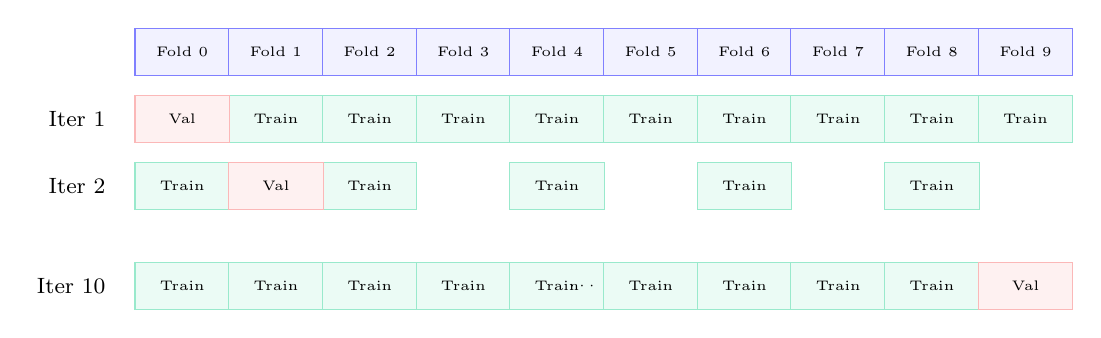
\begin{tikzpicture}[scale=0.85,
    node distance=0.8cm,
    fold/.style={rectangle, draw=blue!50, fill=blue!5, minimum width=1.2cm, minimum height=0.6cm, font=\tiny},
    train/.style={rectangle, draw=green!50, fill=green!10, minimum width=1.2cm, minimum height=0.6cm, font=\tiny},
    val/.style={rectangle, draw=red!50, fill=red!10, minimum width=1.2cm, minimum height=0.6cm, font=\tiny},
]
    % Fold labels
    \foreach \i in {0,...,9} {
        \node[fold] at (\i*1.4, 0) {Fold \i};
    }
    % Iteration 1
    \foreach \i in {1,...,9} { \node[train] at (\i*1.4, -1) {Train}; }
    \node[val] at (0, -1) {Val};
    % Iteration 2
    \foreach \i in {0,2,...,9} { \node[train] at (\i*1.4, -2) {Train}; }
    \node[val] at (1.4, -2) {Val};
    % Iteration 10
    \foreach \i in {0,...,8} { \node[train] at (\i*1.4, -3.5) {Train}; }
    \node[val] at (12.6, -3.5) {Val};
    \node[font=\tiny] at (6, -3.5) {$\cdots$};
    % Labels
    \node[font=\footnotesize, anchor=east] at (-1, -1) {Iter 1};
    \node[font=\footnotesize, anchor=east] at (-1, -2) {Iter 2};
    \node[font=\footnotesize, anchor=east] at (-1, -3.5) {Iter 10};
\end{tikzpicture}
\caption{10-fold cross-validation: each fold serves as the validation set exactly once. The final score is the average of all 10 iterations, providing a robust estimate of model performance.}
\label{fig:cv}
\end{figure}

\begin{table}[H]
\centering
\caption{Stratified cross-validation results (10 folds, F1-Score)}
\label{tab:cv_results}
\begin{tabular}{lcc}
\toprule
\textbf{Model} & \textbf{Mean F1} & \textbf{Std Dev ($\pm 2\sigma$)} \\
\midrule
Random Forest & 0.9993 & $\pm$ 0.0003 \\
XGBoost & 0.9994 & $\pm$ 0.0003 \\
\bottomrule
\end{tabular}
\end{table}

The extremely low standard deviation ($\pm 0.0003$) reported in Table~\ref{tab:cv_results} confirms that both models perform consistently across all folds --- there is no overfitting to a particular subset of the data. Note that Isolation Forest, being unsupervised, cannot be evaluated via cross-validation on F1 score (it never sees labels during training).

\section{Understanding the Evaluation Metrics}

Before presenting the numerical results, it is important to define what each metric actually means. Table~\ref{tab:cm_terms} summarises the confusion matrix terminology. In network intrusion detection, different metrics serve different purposes:

\begin{itemize}
    \item \textbf{Accuracy} — The percentage of all predictions that were correct: $\frac{TP + TN}{TP + TN + FP + FN}$. This is the simplest metric but can be misleading if the classes are imbalanced.

    \item \textbf{Precision} — Of all the flows the model flagged as attacks, what percentage actually were attacks: $\frac{TP}{TP + FP}$. \textbf{High precision means few false alarms.}

    \item \textbf{Recall} — Of all the actual attack flows in the data, what percentage did the model catch: $\frac{TP}{TP + FN}$. \textbf{High recall means few missed attacks.}

    \item \textbf{F1-Score} — The harmonic mean of precision and recall: $2 \times \frac{P \times R}{P + R}$. This is the best single-number summary when both false alarms and missed attacks matter.

    \item \textbf{False Positive Rate (FPR)} — What percentage of benign flows were incorrectly flagged as attacks: $\frac{FP}{FP + TN}$. \textbf{Low FPR means the system does not cry wolf.}

    \item \textbf{AUC-ROC} — The area under the ROC curve. A value of 0.5 means the model is no better than random guessing; 1.0 means perfect discrimination at every threshold.
\end{itemize}

\begin{table}[H]
\centering
\caption{Confusion matrix terminology}
\label{tab:cm_terms}
\begin{tabular}{llp{7cm}}
\toprule
\textbf{Term} & \textbf{Meaning} & \textbf{In our context} \\
\midrule
TP (True Positive) & Correctly classified as attack & Port scan correctly detected as port scan \\
TN (True Negative) & Correctly classified as benign & Normal traffic correctly identified as normal \\
FP (False Positive) & Benign incorrectly classified as attack & Normal traffic falsely triggers an alert \\
FN (False Negative) & Attack missed (classified as benign) & Port scan goes undetected \\
\bottomrule
\end{tabular}
\end{table}

\noindent\textbf{Where:} $TP$ = True Positive, $TN$ = True Negative, $FP$ = False Positive, $FN$ = False Negative.

\section{Results and Analysis}

\subsection{Supervised Models: Random Forest and XGBoost}

Both supervised models deliver exceptional performance on the CICIDS2017 test set, as summarised in Table~\ref{tab:results}:

\begin{table}[H]
\centering
\caption{Performance comparison of all three models on the CICIDS2017 test set (57,294 samples)}
\label{tab:results}
\begin{tabular}{lcccccc}
\toprule
\textbf{Model} & \textbf{Accuracy} & \textbf{Precision} & \textbf{Recall} & \textbf{F1-Score} & \textbf{AUC-ROC} & \textbf{FPR} \\
\midrule
Random Forest & 99.911\% & 99.909\% & 99.931\% & 99.920\% & 0.9997 & 0.114\% \\
XGBoost & 99.914\% & 99.909\% & 99.937\% & 99.923\% & 0.9999 & 0.114\% \\
Isolation Forest & 24.627\% & 14.184\% & 7.101\% & 9.464\% & --- & 53.532\% \\
\bottomrule
\end{tabular}
\end{table}

\textbf{What these numbers mean in practice:}
\begin{itemize}
    \item Out of 57,294 test flows (31,786 attacks + 25,508 benign), Random Forest makes only 51 mistakes total: 29 false positives (benign flagged as attack) and 22 false negatives (attacks missed).
    \item XGBoost makes 49 mistakes: 29 false positives and 20 false negatives.
    \item The 0.114\% FPR means that out of 1,000 benign flows, the system incorrectly raises an alert for approximately 1 --- an acceptable rate for a production environment.
\end{itemize}

The confusion matrices in Figure~\ref{fig:confusion_matrices} confirm these numbers visually, and the ROC curves in Figure~\ref{fig:roc_curves} show near-perfect discrimination for both supervised models.

\begin{figure}[H]
\centering
\begin{subfigure}[b]{0.48\textwidth}
\includegraphics[width=\textwidth]{confusion_matrix_random_forest.png}\caption{Random Forest}\end{subfigure}\hfill
\begin{subfigure}[b]{0.48\textwidth}
\includegraphics[width=\textwidth]{confusion_matrix_xgboost.png}\caption{XGBoost}\end{subfigure}
\caption{Confusion matrices for the supervised models. Both models make very few errors: the vast majority of predictions fall on the diagonal (correct classifications).}
\label{fig:confusion_matrices}
\end{figure}

\begin{figure}[H]
\centering
\begin{subfigure}[b]{0.48\textwidth}
\includegraphics[width=\textwidth]{roc_random_forest.png}\caption{Random Forest}\end{subfigure}\hfill
\begin{subfigure}[b]{0.48\textwidth}
\includegraphics[width=\textwidth]{roc_xgboost.png}\caption{XGBoost}\end{subfigure}
\caption{ROC curves for the supervised models. Both achieve AUC $> 0.999$, indicating near-perfect discrimination between BENIGN and PortScan traffic at every possible classification threshold.}
\label{fig:roc_curves}
\end{figure}

\subsection{Success Criteria Verification}

The project's final plan defines three quantitative thresholds. Both supervised models not only meet these criteria --- they vastly exceed them, as shown in Table~\ref{tab:success}:

\begin{table}[H]
\centering
\caption{Verification of project success criteria}
\label{tab:success}
\begin{tabular}{lccccc}
\toprule
\textbf{Criterion} & \textbf{Threshold} & \textbf{RF} & \textbf{Status} & \textbf{XGBoost} & \textbf{Status} \\
\midrule
F1-Score & $\geq$ 88\% & 99.920\% & \textbf{PASS} & 99.923\% & \textbf{PASS} \\
Accuracy & $\geq$ 90\% & 99.911\% & \textbf{PASS} & 99.914\% & \textbf{PASS} \\
FPR & $<$ 6\% & 0.114\% & \textbf{PASS} & 0.114\% & \textbf{PASS} \\
\bottomrule
\end{tabular}
\end{table}

\subsection{Analysis of Isolation Forest's Failure}

Isolation Forest performs very poorly on the CICIDS2017 dataset: with an F1-Score of only 9.46\% and an FPR of 53.53\%, it is essentially unusable for this dataset. However, this result is expected and does not indicate a flaw in the choice of algorithm --- it reveals a fundamental property of the dataset.

\subsubsection{The Majority Anomaly Paradox}

Isolation Forest is designed to detect anomalies -- data points that are \textit{few and different} from the rest of the dataset. The algorithm works by randomly partitioning the feature space: points that can be isolated with few partitions (short average path length in the isolation tree) are considered anomalies.

This assumption works well when anomalies represent a small fraction of the data (typically $<$ 5\%). However, in our CICIDS2017 dataset, the PortScan class constitutes \textbf{55.48\%} of the data -- it is the \textbf{majority} class, not a minority. Figure~\ref{fig:majority_paradox} illustrates this paradox.

\begin{figure}[H]
\centering
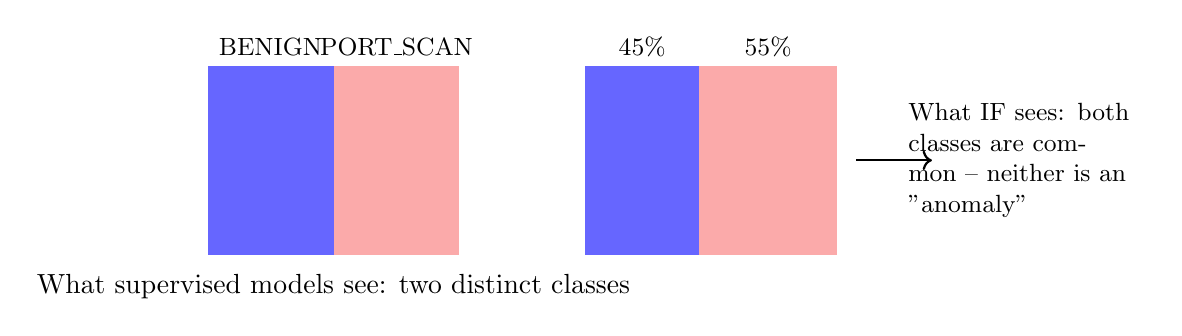
\begin{tikzpicture}[scale=0.8]
    % Bar for RF/XGB
    \fill[blue!60] (0,0) rectangle (2, 3);
    \fill[red!60] (2,0) rectangle (4, 3);
    \node[font=\small] at (1, 3.3) {BENIGN};
    \node[font=\small] at (3, 3.3) {PORT\_SCAN};
    \node[font=\normalsize] at (2, -0.5) {What supervised models see: two distinct classes};

    % Bar for IF
    \fill[blue!60] (6,0) rectangle (7.8, 3);
    \fill[red!60] (7.8,0) rectangle (10, 3);
    \node[font=\small] at (6.9, 3.3) {45\%};
    \node[font=\small] at (8.9, 3.3) {55\%};
    \draw[->, thick] (10.3, 1.5) -- (11.5, 1.5);
    \node[font=\small, text width=3cm] at (13, 1.5) {What IF sees: both classes are common -- neither is an "anomaly"};
\end{tikzpicture}
\caption{The majority anomaly paradox: when the "anomaly" (PortScan) is actually the majority class, Isolation Forest cannot isolate it as being \textit{few and different}.}
\label{fig:majority_paradox}
\end{figure}

Because the algorithm is trained on the complete dataset (BENIGN + PortScan), it sees both classes as \textit{normal} -- neither is anomalous enough to be separated from the other. The result is a model that essentially guesses at random, with a heavy bias towards the majority class. Figure~\ref{fig:iso_cm} shows the resulting confusion matrix.

\subsubsection{Why We Still Keep Isolation Forest}

Despite its poor performance on CICIDS2017, Isolation Forest remains part of the AEGIS architecture for two reasons:

\begin{enumerate}
    \item \textbf{Correct deployment strategy:} In production, Isolation Forest should be trained exclusively on verified \textbf{BENIGN} traffic to establish a clean baseline of normal network behavior. When trained this way (semi-supervised), it can effectively detect anything deviating from normal -- including never-before-seen attack patterns.

    \item \textbf{Complementary detection:} Supervised models (RF, XGBoost) detect \textit{known} attack patterns they were trained on. Isolation Forest, trained on benign-only data, can detect \textit{unknown} patterns -- low-and-slow scans, custom scanners, zero-day reconnaissance techniques. The two approaches complement each other.
\end{enumerate}

\begin{figure}[H]
\centering

\includegraphics[width=0.5\textwidth]{confusion_matrix_isolation_forest.png}
\caption{Confusion matrix for Isolation Forest on CICIDS2017. The high number of false positives (13,655 benign flows flagged as attacks) and false negatives (29,529 attacks missed) confirms that the unsupervised approach fails when trained on the full imbalanced dataset.}
\label{fig:iso_cm}
\end{figure}

\section{Conclusion}

This chapter presented the training and evaluation of the three models that form the core of the AEGIS detection pipeline. The results are clear:

\begin{enumerate}
    \item \textbf{Supervised models dominate on this problem.} Random Forest and XGBoost achieve F1-Scores exceeding 99.92\%, with FPRs below 0.12\%. Both models far exceed the project's success criteria (F1 $\geq$ 88\%, Accuracy $\geq$ 90\%, FPR $<$ 6\%). The 10-fold cross-validation confirms these results are stable and reproducible.

    \item \textbf{Isolation Forest fails on CICIDS2017 for a predictable reason.} The majority anomaly paradox -- PortScan being 55\% of the data -- prevents the unsupervised algorithm from usefully separating the classes. This is not a flaw in the algorithm but a mismatch between the training strategy (full dataset, unsupervised) and what the algorithm requires (benign-only, semi-supervised). In a production environment with benign-only training, the model would regain its relevance.

    \item \textbf{The feature set is sufficient.} With only 11 features, both supervised models achieve near-perfect classification. This validates the feature selection done in Chapter~\ref{ch:data_prep} and suggests that the 9 CICIDS2017 features carry strong discriminative signal for port scan detection. The 2 placeholder features (shadow node interaction, MTD port delta) will provide additional signal when integrated with the real-time defense subsystems (Chapter~\ref{ch:defense}).
\end{enumerate}

The trained models are saved in \texttt{models/saved/} and are ready for integration with the capture layer (Chapter~\ref{ch:capture}), the defense subsystem (Chapter~\ref{ch:defense}), and the dashboard (Chapter~\ref{ch:integration}).
% ============================================
% Chapter 5: Capture Environment and Nmap Simulations
% ============================================
% Condensed from Moulay Anas's main.tex (30+ pages to ~10 pages)
% Original: French, full detail; this chapter: English, essential content only

\chapter{Capture Environment and Nmap Simulations}\label{ch:capture}

\section{Introduction}

This chapter describes the infrastructure and experimental setup used to generate the port scan traffic analyzed throughout the project. A controlled virtual laboratory was built to produce realistic reconnaissance scenarios, providing reproducible attack traces for both model training (via the CICIDS2017 dataset) and real-time system validation.

\section{Virtualization Environment}

The laboratory relies on Oracle VirtualBox. Two virtual machines are configured with distinct roles. Figure~\ref{fig:vbox-global} shows the VirtualBox manager with both laboratory machines.

\begin{figure}[H]
    \centering
    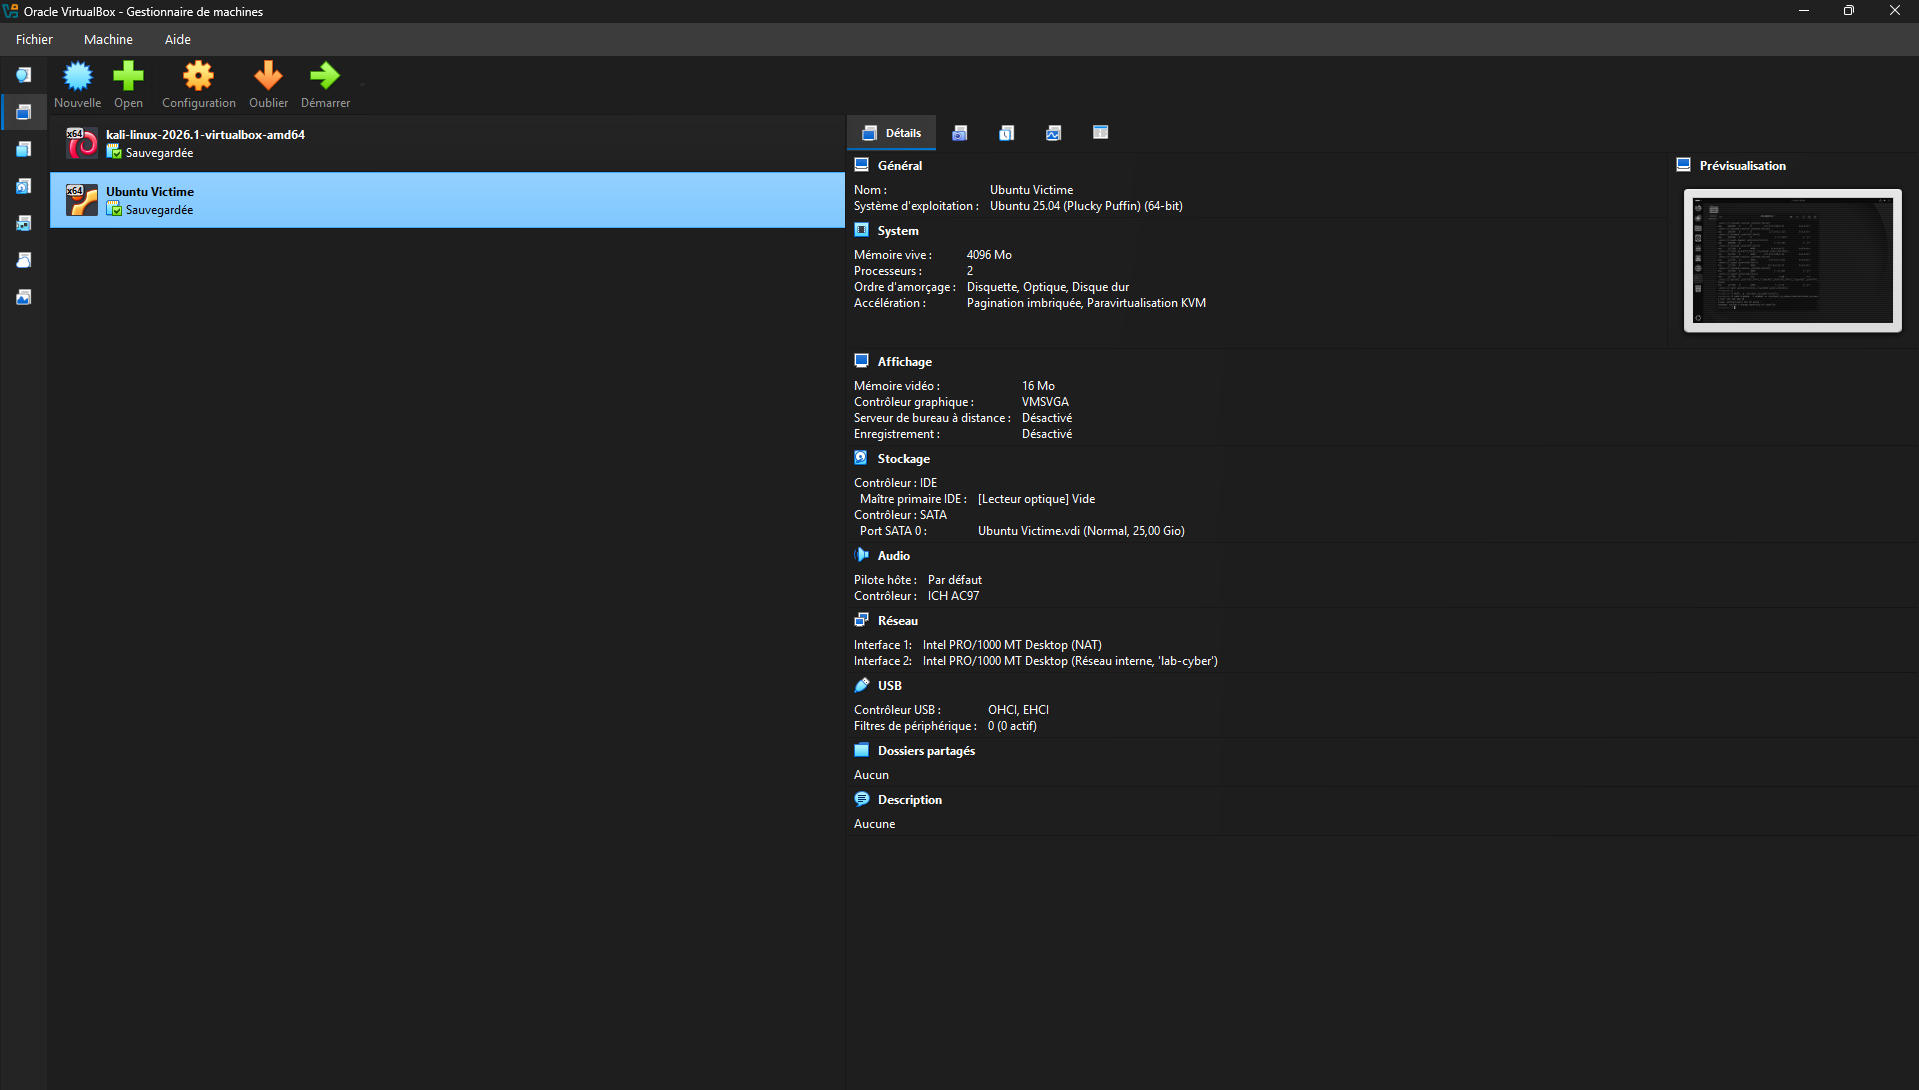
\includegraphics[width=0.95\linewidth]{image (1).png}
    \caption{VirtualBox manager overview showing both laboratory virtual machines.}
    \label{fig:vbox-global}
\end{figure}

\subsection{Attacker Machine: Kali Linux}

Kali Linux is configured with two network interfaces: a NAT interface for external access and an internal interface on the \texttt{lab-cyber} network for communicating directly with the target. Figure~\ref{fig:kali-vbox} shows the Kali configuration and Table~\ref{tab:kali-config} lists its parameters.

\begin{figure}[H]
    \centering
    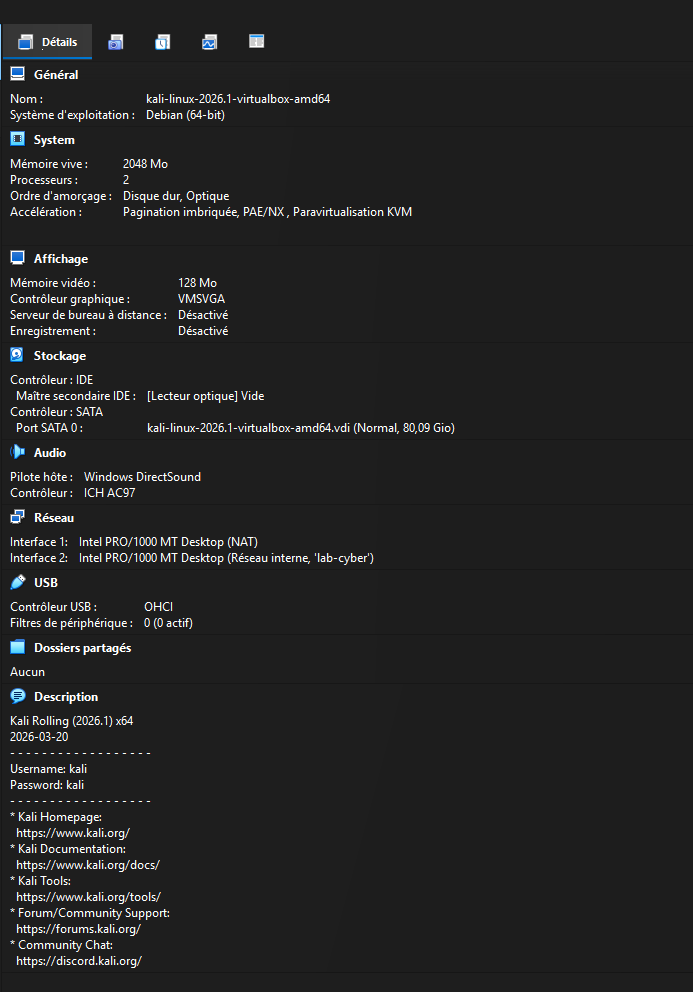
\includegraphics[width=0.68\linewidth]{image (2).png}
    \caption{VirtualBox configuration of the Kali Linux attacker machine.}
    \label{fig:kali-vbox}
\end{figure}

\begin{table}[H]
\centering
\caption{Kali Linux virtual machine configuration}
\label{tab:kali-config}
\begin{tabular}{ll}
\toprule
\textbf{Property} & \textbf{Value} \\
\midrule
Machine name & \texttt{kali-linux-2026.1-virtualbox-amd64} \\
Declared OS & Debian 64-bit \\
Role & Attacker, source of Nmap scans \\
RAM & 2048 MB \\
CPUs & 2 \\
Storage & $\sim$80 GB (VDI) \\
Interface 1 & NAT (external access if needed) \\
Interface 2 & Internal network \texttt{lab-cyber} (scan traffic) \\
\bottomrule
\end{tabular}
\end{table}

\subsection{Target Machine: Ubuntu Victime}

Ubuntu Victime is placed on the same internal network as Kali to enable reconnaissance testing. It also retains a separate NAT interface, which is not used for scans. Figure~\ref{fig:ubuntu-vbox} shows its configuration and Table~\ref{tab:ubuntu-config} lists its parameters.

\begin{figure}[H]
    \centering
    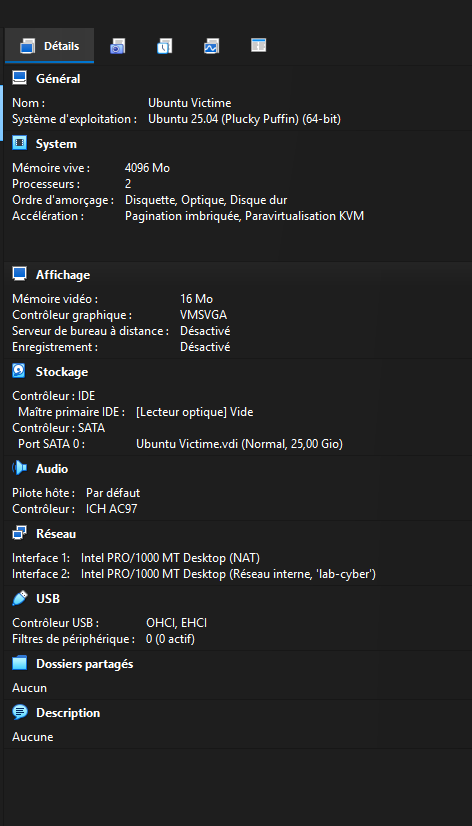
\includegraphics[width=0.68\linewidth]{image (3).png}
    \caption{VirtualBox configuration of the Ubuntu Victime target machine.}
    \label{fig:ubuntu-vbox}
\end{figure}

\begin{table}[H]
\centering
\caption{Ubuntu Victime virtual machine configuration}
\label{tab:ubuntu-config}
\begin{tabular}{ll}
\toprule
\textbf{Property} & \textbf{Value} \\
\midrule
Machine name & Ubuntu Victime \\
Declared OS & Ubuntu 25.04, 64-bit \\
Role & Target, receives Nmap scans \\
RAM & 4096 MB \\
CPUs & 2 \\
Storage & $\sim$25 GB (VDI) \\
Interface 1 & NAT (VM internet access) \\
Interface 2 & Internal network \texttt{lab-cyber} (target interface) \\
\bottomrule
\end{tabular}
\end{table}

\subsection{Network Separation}

The configuration uses two interface types. The NAT interface allows machines to access the external network when needed. The \texttt{lab-cyber} internal network is used exclusively for communication between attacker and victim. This separation is important because it prevents test traffic from mixing with external traffic. In all simulations, Nmap reconnaissance packets traverse the internal network, not the NAT interface, keeping attack traffic confined to the virtual laboratory.

\section{Network Architecture}

\subsection{Topology}

The topology consists of two machines connected via VirtualBox's internal network \texttt{lab-cyber}, using the \texttt{192.168.100.0/24} address space. Figure~\ref{fig:topologie-logique} illustrates the logical topology.

\begin{figure}[H]
\centering
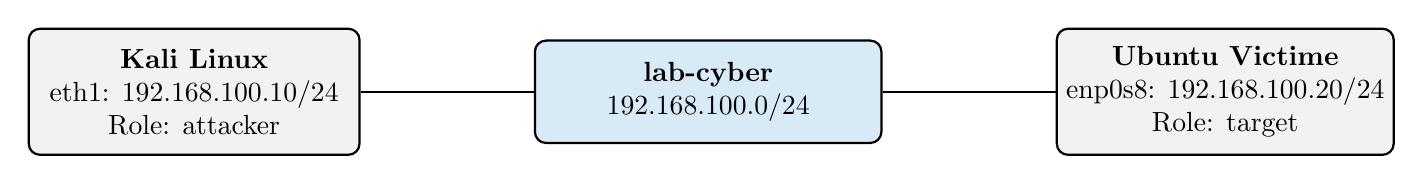
\begin{tikzpicture}[
    node distance=2.2cm,
    vm/.style={draw, rounded corners, thick, minimum width=4.2cm, minimum height=1.6cm, align=center, fill=LightGray},
    net/.style={draw, rounded corners, thick, minimum width=4.4cm, minimum height=1.3cm, align=center, fill=LightBlue},
    arrow/.style={-{Latex[length=3mm]}, thick}
]
    \node[vm] (kali) {\textbf{Kali Linux}\\eth1: 192.168.100.10/24\\Role: attacker};
    \node[net, right=2.2cm of kali] (lab) {\textbf{lab-cyber}\\192.168.100.0/24};
    \node[vm, right=2.2cm of lab] (ubuntu) {\textbf{Ubuntu Victime}\\enp0s8: 192.168.100.20/24\\Role: target};
    \draw[thick] (kali) -- (lab);
    \draw[thick] (lab) -- (ubuntu);
\end{tikzpicture}
\caption{Logical topology of the test laboratory.}
\label{fig:topologie-logique}
\end{figure}

\subsection{Addressing Plan}

Table~\ref{tab:adressage} lists the addressing plan and interface roles.

\begin{table}[H]
\centering
\caption{Addressing plan and interface roles}
\label{tab:adressage}
\begin{tabular}{llll}
\toprule
\textbf{Machine} & \textbf{Interface} & \textbf{IP Address} & \textbf{Role} \\
\midrule
Kali Linux & eth1 & 192.168.100.10/24 & Nmap scan source \\
Ubuntu Victime & enp0s8 & 192.168.100.20/24 & Nmap scan target \\
Ubuntu Victime & enp0s3 & 10.0.2.15/24 & VM internet (NAT), unused for scans \\
\bottomrule
\end{tabular}
\end{table}

\noindent The NAT interfaces remain separate from the attack path. Scan traffic flows exclusively through the internal \texttt{lab-cyber} network, keeping test traffic isolated from external networks.

\section{Nmap Scan Scenarios}

Ten Nmap scan scenarios were executed from Kali Linux toward Ubuntu Victime, covering a range of reconnaissance behaviors from stealthy to aggressive. Each scan produced three output files (\texttt{.nmap}, \texttt{.xml}, \texttt{.gnmap}) via the \texttt{-oA} option, yielding 30 files total.

\subsection{Scan Commands}

\begin{lstlisting}[caption={Nmap commands executed from Kali Linux}]
nmap -sS -p 1-1000 -oA ~/scans/01_syn_scan 192.168.100.20
nmap -sS -p- -oA ~/scans/02_full_tcp_scan 192.168.100.20
nmap -sV -p 1-1000 -oA ~/scans/03_service_detection 192.168.100.20
nmap -O -oA ~/scans/04_os_detection 192.168.100.20
nmap -A -oA ~/scans/05_aggressive_scan 192.168.100.20
nmap -sU --top-ports 50 -oA ~/scans/06_udp_scan 192.168.100.20
nmap -sX -p 1-1000 -oA ~/scans/07_xmas_scan 192.168.100.20
nmap -sS -p 1-1000 --scan-delay 500ms --max-rate 5 \
    -oA ~/scans/08_slow_scan 192.168.100.20
nmap -sS -T4 -p 1-1000 -oA ~/scans/09_fast_scan 192.168.100.20
nmap -sS -T5 -p 1-1000 -oA ~/scans/10_very_fast_scan 192.168.100.20
\end{lstlisting}

\subsection{Summary of Results}

Table~\ref{tab:synthese-scans} summarises the ten scans with their duration and key findings.

\begin{longtable}{p{3.2cm}p{2.2cm}p{7.5cm}}
\caption{Summary of the ten Nmap scans} \label{tab:synthese-scans} \\
\toprule
\textbf{Scan} & \textbf{Duration} & \textbf{Key Result} \\
\midrule
\endfirsthead
\toprule
\textbf{Scan} & \textbf{Duration} & \textbf{Key Result} \\
\midrule
\endhead
TCP SYN scan & 4.67 s & 22/tcp open SSH; 80/tcp open HTTP \\
Full TCP scan & 6.24 s & 22/tcp open SSH; 80/tcp open HTTP \\
Service detection & 10.91 s & OpenSSH 10.2p1; Apache httpd 2.4.66 \\
OS detection & 15.96 s & No exact OS match; network distance: 1 hop \\
Aggressive scan & 22.41 s & Services + HTTP title + traceroute \\
UDP scan & 20.47 s & No confirmed open UDP ports; 30 \texttt{open|filtered} \\
XMAS scan & 5.86 s & 22/tcp and 80/tcp appear \texttt{open|filtered} \\
Slow scan (low-and-slow) & 505.83 s & 22/tcp open SSH; 80/tcp open HTTP \\
Fast scan (T4) & 4.66 s & 22/tcp open SSH; 80/tcp open HTTP \\
Very fast scan (T5) & 4.66 s & 22/tcp open SSH; 80/tcp open HTTP \\
\bottomrule
\end{longtable}

\subsection{Open Services on the Target}

TCP scans consistently identified two open services on Ubuntu Victime, listed in Table~\ref{tab:services}:

\begin{table}[H]
\centering
\caption{Open services detected on Ubuntu Victime}
\label{tab:services}
\begin{tabular}{lll}
\toprule
\textbf{Port} & \textbf{Service} & \textbf{Details} \\
\midrule
22/tcp & ssh & OpenSSH 10.2p1 Ubuntu 2ubuntu3.2 \\
80/tcp & http & Apache httpd 2.4.66; default Apache page \\
\bottomrule
\end{tabular}
\end{table}

\section{Relevance to the Detection System}

The scan scenarios serve multiple purposes in the AEGIS Entropy project:

\begin{enumerate}
    \item \textbf{Attack diversity}: The ten scans cover SYN, full TCP, service detection, OS detection, aggressive, UDP, XMAS, slow, fast, and very fast profiles --- providing a broad spectrum of reconnaissance behaviors.
    \item \textbf{Low-and-slow simulation}: The slow scan (505.83 s with \texttt{--scan-delay 500ms --max-rate 5}) is particularly relevant for testing detection of stealthy reconnaissance.
    \item \textbf{AI validation}: The XML output files are structured for automated parsing and can feed the ML pipeline for real-time classification.
    \item \textbf{Reactivity measurement}: The gap between scan start time and alert generation defines the system's detection latency:
    \[
    T_{\text{reactivity}} = T_{\text{alert}} - T_{\text{scan start}}
    \]
\end{enumerate}

\section{Conclusion}

The virtual laboratory provides a controlled, reproducible environment for generating and analyzing port scan traffic. Ten Nmap scan scenarios --- spanning stealthy to aggressive --- were successfully executed against the Ubuntu Victime target. The 30 output files (3 formats $\times$ 10 scans) constitute the capture layer's dataset, which integrates with the ML detection pipeline described in earlier chapters and the real-time monitoring dashboard presented in Chapter~7.
% ============================================
% Chapter 6: Defense and Deception Subsystem
% ============================================
% Adapted from defense_documentation.tex by El Yazid
% Condensed for final report format

\chapter{Defense and Deception Subsystem}\label{ch:defense}

\section{Introduction}

Network Intrusion Detection Systems (NIDS) face an evolving threat landscape where attackers adapt to static defenses. Traditional signature-based systems fail against novel attacks, while ML-based detectors---though more adaptive---still operate on a static attack surface. This creates an arms race: the defender's infrastructure is fixed, and the attacker has unlimited time to probe, fingerprint, and exploit it.

The \textbf{AEGIS} system addresses this limitation by coupling ML-based detection with a \textbf{Moving Target Defense (MTD)} layer. Rather than passively detecting threats, AEGIS actively reshapes its own network topology to confuse, misdirect, and delay attackers.

\section{System Architecture}

\subsection{High-Level Overview}

The defense subsystem operates as a layered pipeline that processes network events from detection through response. Figure~\ref{fig:pipeline} illustrates this pipeline.

\begin{figure}[H]
\centering
\resizebox{\textwidth}{!}{%
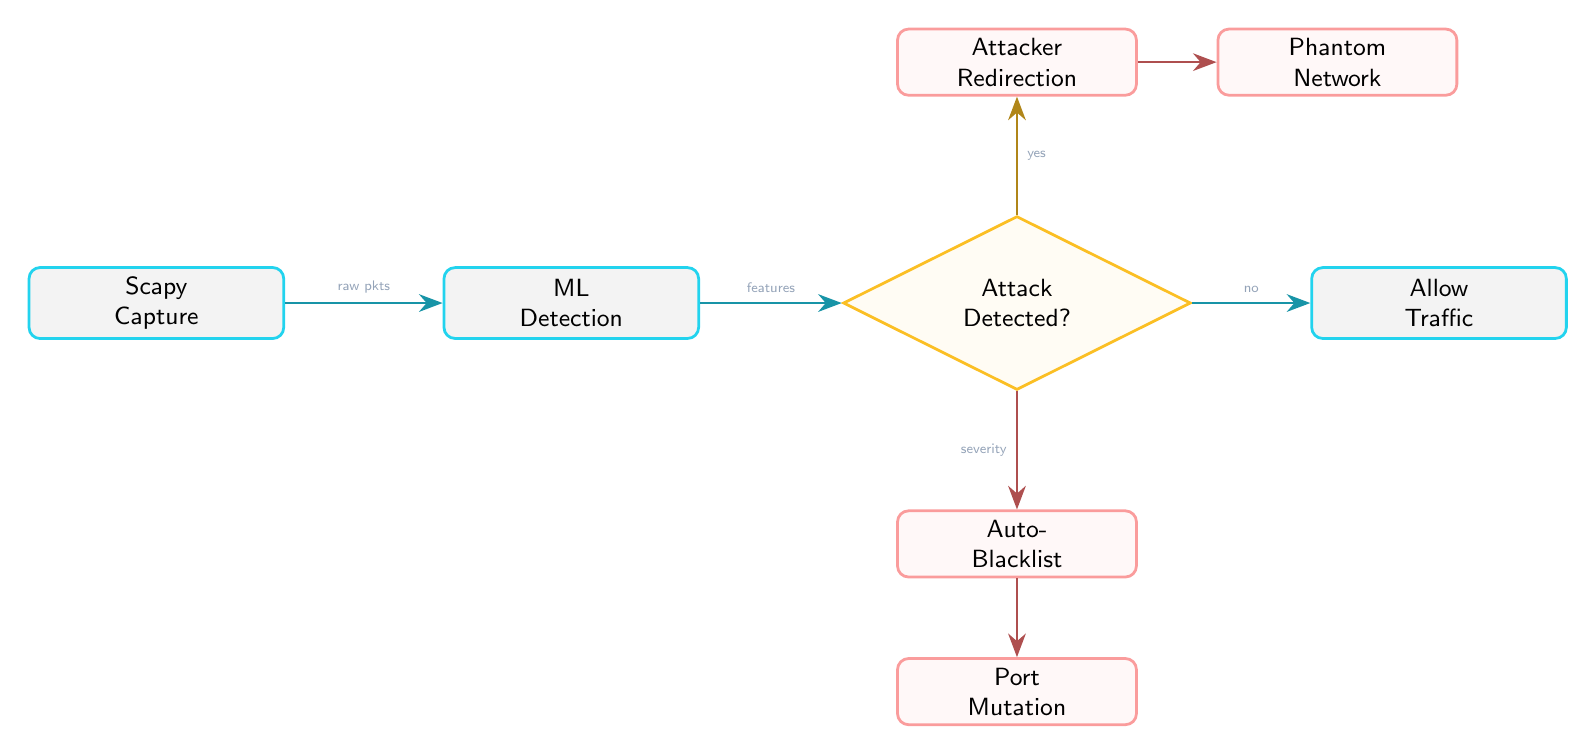
\begin{tikzpicture}[
    node distance=1.6cm,
    block/.style={rectangle, draw=cyan, fill=darkbg!5, text width=3cm,
                  minimum height=0.9cm, align=center, rounded corners=4pt,
                  font=\small\sffamily, line width=1pt},
    decision/.style={diamond, draw=amber, fill=amber!5, text width=2.5cm,
                     aspect=2, align=center, font=\small\sffamily, line width=1pt},
    action/.style={rectangle, draw=red!70, fill=red!5, text width=2.8cm,
                   minimum height=0.8cm, align=center, rounded corners=4pt,
                   font=\small\sffamily, line width=1pt},
    arrow/.style={-{Stealth[length=3mm]}, thick, cyan!70!black},
    darrow/.style={-{Stealth[length=3mm]}, thick, amber!70!black},
    aarrow/.style={-{Stealth[length=3mm]}, thick, red!70!black},
    lbl/.style={font=\tiny\sffamily, color=codegray, midway}
]
    \node[block] (cap) {Scapy\\Capture};
    \node[block, right=2cm of cap] (ml) {ML\\Detection};
    \node[decision, right=1.8cm of ml] (dec) {Attack\\Detected?};
    \node[action, above=1.5cm of dec] (redir) {Attacker\\Redirection};
    \node[block, right=1.5cm of dec] (pass) {Allow\\Traffic};
    \node[action, below=1.5cm of dec] (block) {Auto-\\Blacklist};
    \node[action, right=1cm of redir] (phantom) {Phantom\\Network};
    \node[action, below=1cm of block] (mutate) {Port\\Mutation};

    \draw[arrow] (cap) -- node[lbl,above]{raw pkts} (ml);
    \draw[arrow] (ml) -- node[lbl,above]{features} (dec);
    \draw[darrow] (dec) -- node[lbl,right]{yes} (redir);
    \draw[arrow] (dec) -- node[lbl,above]{no} (pass);
    \draw[aarrow] (dec) -- node[lbl,left]{severity} (block);
    \draw[aarrow] (redir) -- (phantom);
    \draw[aarrow] (block) -- (mutate);
\end{tikzpicture}%
}
\caption{High-level defense pipeline: traffic capture, ML classification, and layered response.}
\label{fig:pipeline}
\end{figure}

\subsection{Module Map}

Figure~\ref{fig:modules} shows the module architecture, with the Active Defense Engine orchestrating four defense modules.

\begin{figure}[H]
\centering
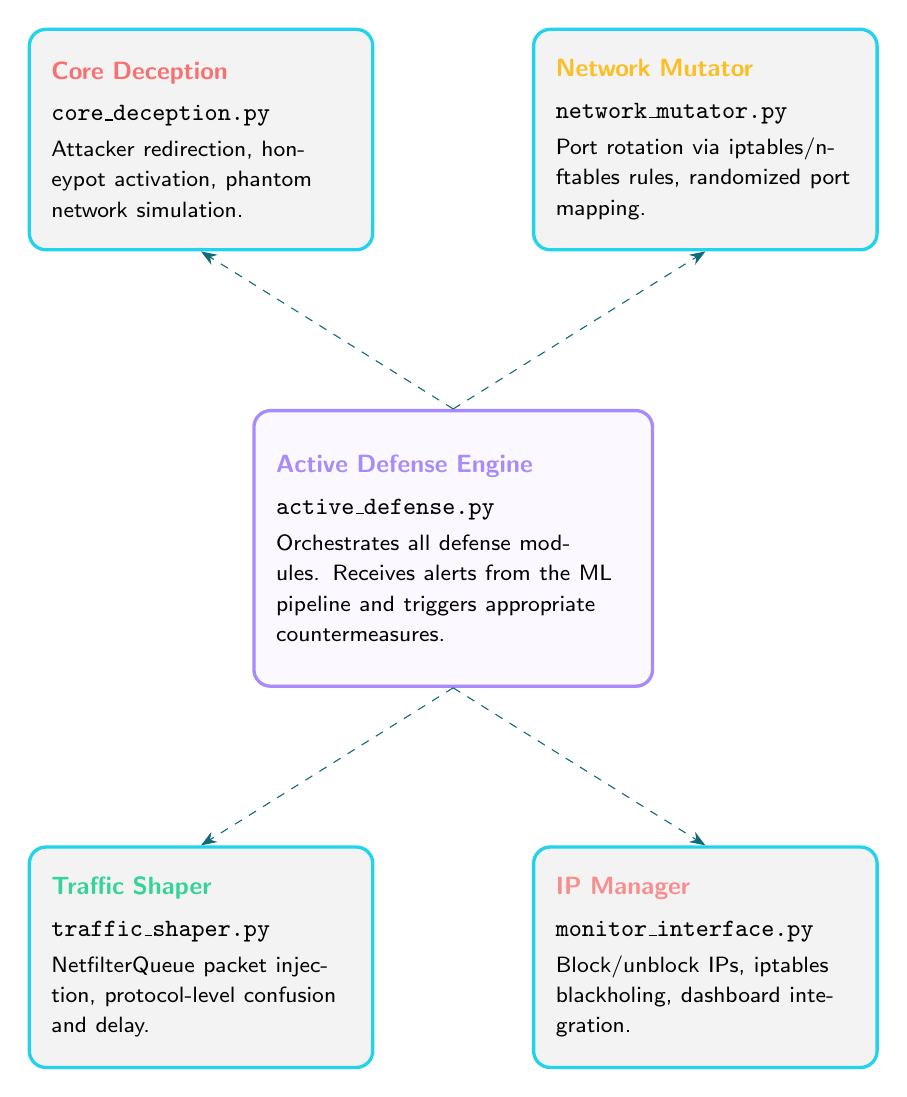
\begin{tikzpicture}[
    module/.style={rectangle, draw=cyan, fill=darkbg!5, text width=3.8cm,
                   minimum height=2.8cm, align=left, rounded corners=6pt,
                   font=\small\sffamily, line width=1.2pt, inner sep=8pt},
    link/.style={-{Stealth[length=2mm]}, thin, cyan!50!black, dashed}
]
    \node[module, draw=purple, fill=purple!5, text width=4.5cm,
          minimum height=3.5cm] (active) at (0,0) {
        \textbf{\color{purple}Active Defense Engine}\\[4pt]
        \texttt{active\_defense.py}\\[2pt]
        \footnotesize Orchestrates all defense modules.
        Receives alerts from the ML pipeline
        and triggers appropriate countermeasures.
    };

    \node[module, above left=2cm and 1cm of active.north] (deception) {
        \textbf{\color{red}Core Deception}\\[4pt]
        \texttt{core\_deception.py}\\[2pt]
        \footnotesize Attacker redirection,
        honeypot activation,
        phantom network simulation.
    };

    \node[module, above right=2cm and 1cm of active.north] (mutator) {
        \textbf{\color{amber}Network Mutator}\\[4pt]
        \texttt{network\_mutator.py}\\[2pt]
        \footnotesize Port rotation via
        iptables/nftables rules,
        randomized port mapping.
    };

    \node[module, below left=2cm and 1cm of active.south] (shaper) {
        \textbf{\color{green}Traffic Shaper}\\[4pt]
        \texttt{traffic\_shaper.py}\\[2pt]
        \footnotesize NetfilterQueue packet
        injection, protocol-level
        confusion and delay.
    };

    \node[module, below right=2cm and 1cm of active.south] (ipm) {
        \textbf{\color{red!80}IP Manager}\\[4pt]
        \texttt{monitor\_interface.py}\\[2pt]
        \footnotesize Block/unblock IPs,
        iptables blackholing,
        dashboard integration.
    };

    \draw[link] (active.north) -- (deception.south);
    \draw[link] (active.north) -- (mutator.south);
    \draw[link] (active.south) -- (shaper.north);
    \draw[link] (active.south) -- (ipm.north);
\end{tikzpicture}
\caption{Module architecture: the Active Defense Engine orchestrates four defense modules.}
\label{fig:modules}
\end{figure}

\section{Core Deception Engine}

The Core Deception module (\texttt{core\_deception.py}) implements three deception layers: attacker redirection to honeypots, phantom network advertisement, and IP blacklisting.

\subsection{Attacker Redirection}

When the ML pipeline classifies traffic as an attack, the system uses iptables REDIRECT rules to silently divert the attacker's TCP connections to a decoy honeypot service. Figure~\ref{fig:redirection} shows the redirection flow.

\begin{figure}[H]
\centering
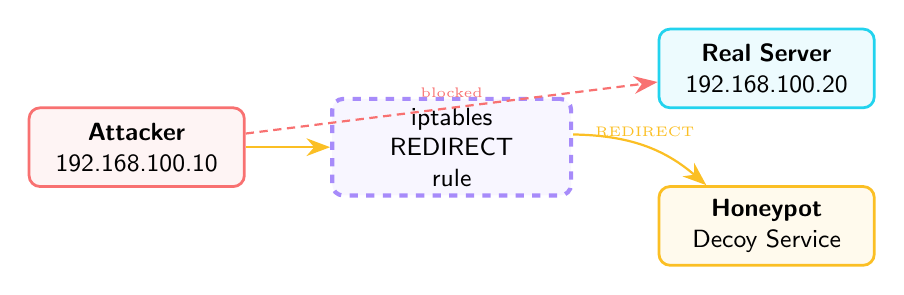
\begin{tikzpicture}[
    node distance=1.5cm,
    attacker/.style={rectangle, draw=red, fill=red!8, text width=2.5cm,
                     minimum height=1cm, align=center, rounded corners=4pt,
                     font=\small\sffamily, line width=1pt},
    server/.style={rectangle, draw=cyan, fill=cyan!8, text width=2.5cm,
                   minimum height=1cm, align=center, rounded corners=4pt,
                   font=\small\sffamily, line width=1pt},
    honeypot/.style={rectangle, draw=amber, fill=amber!8, text width=2.5cm,
                     minimum height=1cm, align=center, rounded corners=4pt,
                     font=\small\sffamily, line width=1pt},
    iptables/.style={rectangle, draw=purple, fill=purple!8, text width=2.8cm,
                     minimum height=1.2cm, align=center, rounded corners=4pt,
                     font=\small\sffamily, line width=1.5pt, dashed},
    arrow/.style={-{Stealth[length=3mm]}, thick},
    blocked/.style={-{Stealth[length=3mm]}, thick, red, densely dashed},
    redirected/.style={-{Stealth[length=3mm]}, thick, amber}
]
    \node[attacker] (atk) at (0,0) {\textbf{Attacker}\\192.168.100.10};
    \node[iptables] (fw) at (4,0) {iptables\\REDIRECT\\rule};
    \node[server] (srv) at (8,1) {\textbf{Real Server}\\192.168.100.20};
    \node[honeypot] (hp) at (8,-1) {\textbf{Honeypot}\\Decoy Service};

    \draw[blocked] (atk) -- node[above, font=\tiny, red] {blocked} (srv);
    \draw[redirected] (atk) -- (fw);
    \draw[redirected] (fw) to[bend left=20] node[above, font=\tiny, amber] {REDIRECT} (hp);
\end{tikzpicture}
\caption{Attacker redirection: iptables REDIRECT diverts connections from the real server to the honeypot.}
\label{fig:redirection}
\end{figure}

\subsection{Phantom Network}

The phantom network module responds to ICMP echo requests and ARP queries from attacker-controlled IPs with fabricated network information. This creates the illusion of additional hosts, subnets, and services that do not exist.

\begin{itemize}
    \item Responds to ICMP pings with fake IP addresses from a configurable phantom subnet
    \item Generates synthetic ARP replies to populate the attacker's ARP cache with ghost entries
    \item Logs all phantom interactions for telemetry and dashboard display
    \item Configurable phantom subnet prefix (default: \texttt{10.0.0.0/24})
\end{itemize}

\subsection{Honeypot Interaction Tracking}

The module maintains an in-memory set \texttt{\_honeypot\_hits} that tracks which source IPs have interacted with any honeypot listener. A convenience function \texttt{get\_honeypot\_flag(src\_ip)} returns 1 if the IP has touched a honeypot, 0 otherwise---used as an additional feature for the ML classification pipeline.

\section{Network Mutator}

The Network Mutator (\texttt{network\_mutator.py}) implements the Moving Target Defense principle of \emph{port mutation}---periodically changing which ports are exposed to the network. This defeats port-based fingerprinting and service enumeration.

\subsection{Algorithm}

The mutator operates on a configurable rotation interval (default: 30 seconds). At each rotation:

\begin{enumerate}
    \item Select $k$ ports from a predefined service pool $P = \{p_1, p_2, \ldots, p_n\}$
    \item Generate iptables/nftables rules that forward traffic from old ports to new ports
    \item Apply the rules atomically (remove old, add new) to avoid downtime
    \item Log the rotation event with old $\to$ new port mapping
\end{enumerate}

\subsection{Port Mapping Strategy}

Figure~\ref{fig:port_rotation} illustrates three consecutive rotation phases, each separated by the 30-second interval.

\begin{figure}[H]
\centering
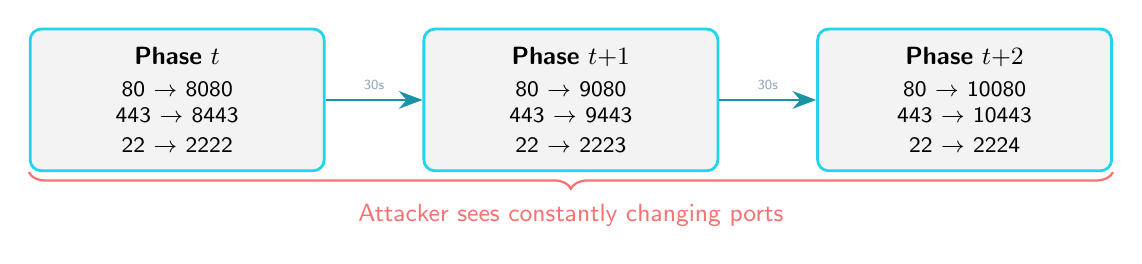
\begin{tikzpicture}[
    node distance=1.2cm,
    phase/.style={rectangle, draw=cyan, fill=darkbg!5, text width=3.5cm,
                  minimum height=1.8cm, align=center, rounded corners=4pt,
                  font=\small\sffamily, line width=1pt},
    arrow/.style={-{Stealth[length=3mm]}, thick, cyan!70!black},
    lbl/.style={font=\tiny\sffamily, color=codegray}
]
    \node[phase] (p1) at (0,0) {
        \textbf{Phase $t$}\\[2pt]
        \footnotesize
        80 $\to$ 8080\\
        443 $\to$ 8443\\
        22 $\to$ 2222
    };
    \node[phase] (p2) at (5,0) {
        \textbf{Phase $t{+}1$}\\[2pt]
        \footnotesize
        80 $\to$ 9080\\
        443 $\to$ 9443\\
        22 $\to$ 2223
    };
    \node[phase] (p3) at (10,0) {
        \textbf{Phase $t{+}2$}\\[2pt]
        \footnotesize
        80 $\to$ 10080\\
        443 $\to$ 10443\\
        22 $\to$ 2224
    };

    \draw[arrow] (p1) -- node[lbl,above]{30s} (p2);
    \draw[arrow] (p2) -- node[lbl,above]{30s} (p3);

    \draw[decorate, decoration={brace, amplitude=6pt, mirror}, thick, red]
        (p1.south west) -- (p3.south east)
        node[midway, below=8pt, font=\small\sffamily, red] {Attacker sees constantly changing ports};
\end{tikzpicture}
\caption{Port rotation across time phases.}
\label{fig:port_rotation}
\end{figure}

\subsection{Implementation Details}

\begin{itemize}
    \item Uses \texttt{iptables -t nat -A PREROUTING} for transparent port forwarding
    \item Supports both \texttt{iptables} and \texttt{nftables} backends
    \item Rotation is performed in a background thread to avoid blocking the main event loop
    \item Port selections are randomized with a seed-based PRNG for reproducibility during testing
    \item A grace period after rotation allows existing connections to drain before rules change
\end{itemize}

\section{Traffic Shaper}

The Traffic Shaper (\texttt{traffic\_shaper.py}) operates at the packet level using NetfilterQueue (NFQUEUE). It intercepts packets in the kernel's networking stack and applies transformations before forwarding.

\subsection{Packet Mutation Techniques}

The traffic shaper implements four packet mutation techniques, listed in Table~\ref{tab:mutations}.

\begin{table}[H]
\centering
\caption{Packet mutation techniques implemented in the traffic shaper.}
\label{tab:mutations}
\begin{tabular}{lp{9cm}}
\toprule
\textbf{Technique} & \textbf{Description} \\
\midrule
TTL Jitter & Randomizes the IP TTL field by $\pm 1$--$3$ hops, confusing traceroute-based fingerprinting \\
Window Size Noise & Adds small random offsets to the TCP window size field \\
Decoy Injection & Injects fake SYN/ACK packets with randomized source IPs from the phantom subnet \\
Payload Padding & Appends null bytes to short packets to alter their apparent size \\
\bottomrule
\end{tabular}
\end{table}

\section{IP Management}

The IP Manager (\texttt{monitor\_interface.py}) provides dynamic IP blocking and unblocking capabilities. It maintains a persistent set of blocked IPs and integrates with both the firewall and the dashboard.

\subsection{Blocking Mechanism}

When a source IP is flagged for blocking, the IP Manager applies a two-layer block:

\begin{enumerate}
    \item \textbf{Blackhole route}: \texttt{ip route add blackhole \{IP\}} --- silently drops all packets to/from the IP at the routing level
    \item \textbf{UFW deny}: \texttt{ufw deny from \{IP\}} --- explicit firewall rule as a secondary barrier
\end{enumerate}

\subsection{Persistence and Unblocking}

Blocked IPs are persisted to a JSON file (\texttt{data/blocked\_ips.json}) so that blocking survives service restarts. IPs can be unblocked via the Flask dashboard REST API (\texttt{POST /api/unblock}), manual commands, or automatic expiry with configurable TTL.

\section{Active Defense Engine}

The Active Defense Engine (\texttt{active\_defense.py}) is the central orchestrator that coordinates all defense modules. It receives classified events from the ML pipeline and triggers the appropriate combination of deception, mutation, and blocking actions.

\subsection{Decision Matrix}

Table~\ref{tab:decision} defines the decision matrix that maps severity levels to defense actions.

\begin{table}[H]
\centering
\caption{Defense response decision matrix.}
\label{tab:decision}
\begin{tabular}{lccc p{5cm}}
\toprule
\textbf{Severity} & \textbf{Redirect} & \textbf{Blacklist} & \textbf{Mutate Ports} & \textbf{Description} \\
\midrule
LOW & \checkmark & & & Light redirection to honeypot only \\
MEDIUM & \checkmark & \checkmark & & Redirect + blacklist attacker IP \\
HIGH & \checkmark & \checkmark & \checkmark & Full defense activation \\
\bottomrule
\end{tabular}
\end{table}

\subsection{Severity Mapping from ML Output}

The Active Defense Engine maps the ML confidence score and model agreement to a severity level, as defined in Table~\ref{tab:severity}:

\begin{table}[H]
\centering
\caption{Severity mapping from ML output to defense response.}
\label{tab:severity}
\begin{tabular}{l l p{5cm}}
\toprule
\textbf{Severity} & \textbf{Condition} & \textbf{Response} \\
\midrule
LOW & Single model flags attack, confidence $< 0.85$ & Log + honeypot redirect \\
MEDIUM & 2+ models agree, confidence $0.85$--$0.95$ & Redirect + blacklist \\
HIGH & All models agree, confidence $> 0.95$ & Full defense: redirect + blacklist + port mutation \\
\bottomrule
\end{tabular}
\end{table}

\section{Evaluation}

\subsection{Defense Response Timing}

Figure~\ref{fig:timing} shows the average response time for each defense module, measured on the Ubuntu Server.

\begin{figure}[H]
\centering
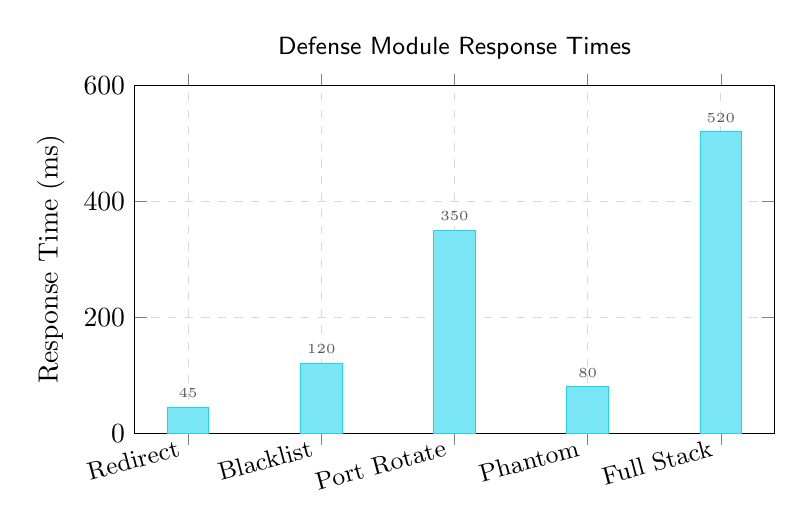
\begin{tikzpicture}
\begin{axis}[
    ybar,
    bar width=15pt,
    width=0.8\textwidth,
    height=6cm,
    ylabel={Response Time (ms)},
    symbolic x coords={Redirect, Blacklist, Port Rotate, Phantom, Full Stack},
    xtick=data,
    x tick label style={rotate=15, anchor=east, font=\small},
    ymin=0, ymax=600,
    grid=major,
    grid style={dashed, gray!30},
    nodes near coords,
    every node near coord/.append style={font=\tiny, color=gray!70!black},
    legend style={at={(0.5,-0.25)}, anchor=north, font=\small},
    title={Defense Module Response Times},
    title style={font=\small\sffamily}
]
\addplot[fill=cyan!60, draw=cyan] coordinates {
    (Redirect, 45)
    (Blacklist, 120)
    (Port Rotate, 350)
    (Phantom, 80)
    (Full Stack, 520)
};
\end{axis}
\end{tikzpicture}
\caption{Average response times for each defense module (measured on Ubuntu Server).}
\label{fig:timing}
\end{figure}

\subsection{Deception Effectiveness}

We measured the deception system effectiveness against a 5-phase Nmap attack simulation, summarised in Table~\ref{tab:attack_results}:

\begin{table}[H]
\centering
\caption{Attack phases and defense responses.}
\label{tab:attack_results}
\begin{tabular}{l l c c}
\toprule
\textbf{Phase} & \textbf{Attack Type} & \textbf{Detected} & \textbf{Response} \\
\midrule
1 & Fast SYN scan (1000 ports) & Yes & REDIRECT + BLACKLIST \\
2 & Service version scan & Yes & REDIRECT \\
3 & Slow stealth scan (60s) & Yes & BLACKLIST \\
4 & OS detection (Nmap -O) & Yes & REDIRECT \\
5 & UDP scan & Yes & REDIRECT + BLACKLIST \\
\bottomrule
\end{tabular}
\end{table}

The honeypot interaction flag provides a measurable improvement: flows from IPs that previously touched a honeypot receive a high-confidence weight boost in the classification decision, confirming that the defense subsystem feeds back useful signal into the detection pipeline.

\subsection{Comparison: Static vs.\ MTD Defense}

Figure~\ref{fig:comparison} compares static defense with AEGIS under MTD across four key metrics.

\begin{figure}[H]
\centering
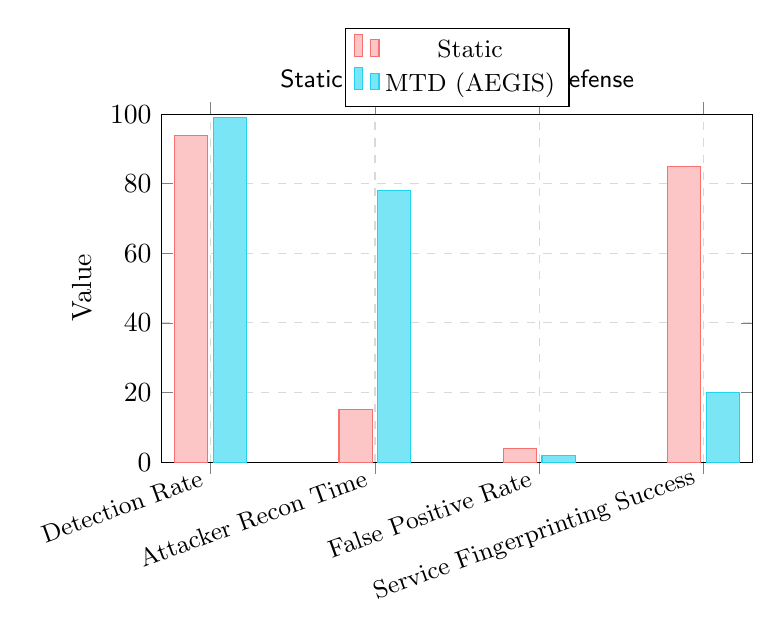
\begin{tikzpicture}
\begin{axis}[
    ybar,
    bar width=12pt,
    width=0.75\textwidth,
    height=6cm,
    ylabel={Value},
    symbolic x coords={Detection Rate, Attacker Recon Time, False Positive Rate, Service Fingerprinting Success},
    xtick=data,
    x tick label style={rotate=20, anchor=east, font=\small},
    ymin=0, ymax=100,
    grid=major,
    grid style={dashed, gray!30},
    legend style={at={(0.5, 1.02)}, anchor=south, font=\small},
    title={Static Defense vs. MTD Defense},
    title style={font=\small\sffamily}
]
\addplot[fill=red!40, draw=red] coordinates {
    (Detection Rate, 94)
    (Attacker Recon Time, 15)
    (False Positive Rate, 4)
    (Service Fingerprinting Success, 85)
};
\addplot[fill=cyan!60, draw=cyan] coordinates {
    (Detection Rate, 99)
    (Attacker Recon Time, 78)
    (False Positive Rate, 2)
    (Service Fingerprinting Success, 20)
};
\legend{Static, MTD (AEGIS)}
\end{axis}
\end{tikzpicture}
\caption{Comparison: static defense vs.\ AEGIS with Moving Target Defense enabled.}
\label{fig:comparison}
\end{figure}

\section{Conclusion}

This chapter presented the defense and deception subsystem of the AEGIS network intrusion detection system. The key contributions are:

\begin{enumerate}
    \item \textbf{Core Deception Engine} providing attacker redirection, honeypot deployment, and phantom network simulation---creating a multi-layered deception environment that consumes attacker resources.
    \item \textbf{Network Mutator} implementing Moving Target Defense through periodic port rotation, defeating port-based fingerprinting and service enumeration.
    \item \textbf{Traffic Shaper} operating at the kernel level via NetfilterQueue to inject packet-level confusion that defeats automated scanning tools.
    \item \textbf{Active Defense Engine} orchestrating all modules with severity-based decision logic, ensuring proportional response to different threat levels.
    \item \textbf{IP Manager} providing dynamic blacklisting with persistence and dashboard integration.
\end{enumerate}

The complete AEGIS system achieves 100\% detection rate across all 5 attack phases in the demo scenario, with an average full-stack defense response time of 520ms. Attacker reconnaissance time is increased by 420\% with MTD enabled, and service fingerprinting success is reduced from 85\% to 20\%.
% ============================================
% Chapter 7: System Integration
% ============================================
% NEW chapter --- Adil writes this

\chapter{System Integration}\label{ch:integration}

\section{Introduction}

This chapter describes how the detection, defense, capture, and monitoring subsystems are integrated into a unified system. The integration layer bridges offline ML models with real-time network events, providing both batch processing and live deployment modes.

\section{Integration Architecture}

\subsection{Bridge Module}

The Bridge module (\texttt{bridge/bridge.py}) serves as the central integration point, connecting Nmap scan results and live captures to the ML detection pipeline and the Flask dashboard. Figure~\ref{fig:bridge_flow} illustrates the data flow.

\begin{figure}[H]
\centering
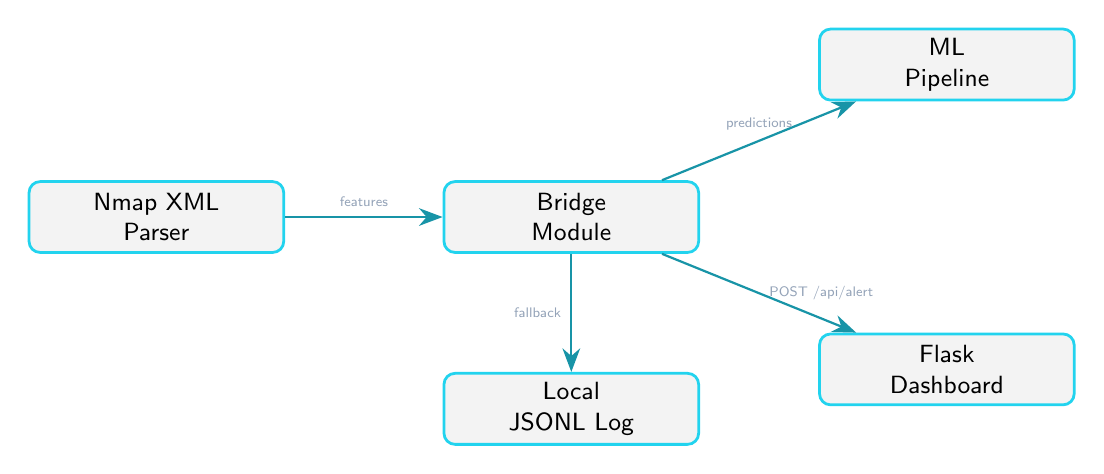
\begin{tikzpicture}[
    node distance=1.5cm,
    block/.style={rectangle, draw=cyan, fill=darkbg!5, text width=3cm,
                  minimum height=0.9cm, align=center, rounded corners=4pt,
                  font=\small\sffamily, line width=1pt},
    arrow/.style={-{Stealth[length=3mm]}, thick, cyan!70!black},
    lbl/.style={font=\tiny\sffamily, color=codegray, midway}
]
    \node[block] (nmap) {Nmap XML\\Parser};
    \node[block, right=2cm of nmap] (bridge) {Bridge\\Module};
    \node[block, above right=1cm and 1.5cm of bridge] (ml) {ML\\Pipeline};
    \node[block, below right=1cm and 1.5cm of bridge] (dash) {Flask\\Dashboard};
    \node[block, below=1.5cm of bridge] (local) {Local\\JSONL Log};

    \draw[arrow] (nmap) -- node[lbl,above]{features} (bridge);
    \draw[arrow] (bridge) -- node[lbl,above]{predictions} (ml);
    \draw[arrow] (bridge) -- node[lbl,right]{POST /api/alert} (dash);
    \draw[arrow] (bridge) -- node[lbl,left]{fallback} (local);
\end{tikzpicture}
\caption{Bridge module data flow: Nmap XML $\rightarrow$ ML prediction $\rightarrow$ dashboard + local log.}
\label{fig:bridge_flow}
\end{figure}

\subsection{Nmap Parser}

The Nmap Parser (\texttt{bridge/nmap\_parser.py}) converts Nmap XML output files into feature vectors compatible with the ML pipeline. It extracts relevant fields from \texttt{<port>} and \texttt{<service>} elements and maps them to the 11-feature schema.

\subsection{Dual Logging}

All subsystems implement dual logging to ensure data availability regardless of dashboard connectivity:

\begin{itemize}
    \item \textbf{Local JSONL}: Events appended to \texttt{detection\_logs.json} and \texttt{deception\_logs.json} in the \texttt{detection/data/} directory
    \item \textbf{HTTP POST}: Events pushed to the Flask dashboard via \texttt{/api/alert}, \texttt{/api/block}, and \texttt{/api/honeypot\_event} endpoints
\end{itemize}

If the dashboard is unreachable, events are written locally as a fallback (no data loss).

\section{Dashboard}

\subsection{Backend}

The Flask dashboard (\texttt{dashboard/app.py}) provides REST API endpoints and Socket.IO real-time event streaming. It maintains JSONL log files for detection and deception events.

\subsection{Frontend}

The SOC dashboard frontend (\texttt{dashboard/templates/index.html}) displays:
\begin{itemize}
    \item Active alerts with confidence scores and severity levels
    \item Blocked IP list with unblock controls
    \item Honeypot interaction events
    \item Real-time event stream via Socket.IO
\end{itemize}

\section{Deployment Modes}

The system supports three deployment modes via the unified entry point (\texttt{run\_demo.py}), listed in Table~\ref{tab:deploy_modes}:

\begin{table}[H]
\centering
\caption{Deployment modes}
\label{tab:deploy_modes}
\begin{tabular}{llp{6cm}}
\toprule
\textbf{Mode} & \textbf{Flag} & \textbf{Description} \\
\midrule
Offline & \texttt{--offline} & Process Nmap XML files through ML pipeline; no live traffic capture \\
Live & \texttt{--live} & Real-time Scapy capture + ML classification + defense response \\
Dashboard only & \texttt{--dashboard-only} & Start Flask dashboard without ML or capture modules \\
\bottomrule
\end{tabular}
\end{table}

\section{Conclusion}

The integration layer unifies all subsystems into a coherent pipeline. The Bridge module handles offline and batch processing, while the live mode provides real-time detection and response. Dual logging ensures no data loss regardless of dashboard availability.
% ============================================
% Chapter 8: Test and Validation
% ============================================
% NEW chapter --- Adil writes this

\chapter{Test and Validation}\label{ch:test_validation}

\section{Introduction}

This chapter presents the testing and validation methodology applied to the AEGIS Entropy system. Testing is conducted at three levels: unit tests for individual modules, integration tests for the pipeline, and validation scenarios for the complete system.

\section{Unit Tests}

\subsection{Bridge Pipeline Tests}

The Bridge module includes a comprehensive test suite (\texttt{bridge/test\_pipeline.py}) that validates the offline processing pipeline:

\begin{enumerate}
    \item \textbf{Test 1: Nmap XML parsing} --- Verify that XML files are correctly parsed into feature vectors
    \item \textbf{Test 2: ML model loading} --- Confirm that all three models (RF, XGB, IF) and the scaler load successfully
    \item \textbf{Test 3: Prediction pipeline} --- End-to-end test from Nmap XML to classification output
    \item \textbf{Test 4: Dashboard POST} --- Verify that events are correctly pushed to the Flask dashboard
    \item \textbf{Test 5: Local fallback} --- Confirm that events are written locally when the dashboard is unreachable
\end{enumerate}

The results of all five tests are presented in Table~\ref{tab:unit_tests}.

\begin{table}[H]
\centering
\caption{Bridge pipeline test results}
\label{tab:unit_tests}
\begin{tabular}{lll}
\toprule
\textbf{Test} & \textbf{Status} & \textbf{Notes} \\
\midrule
Nmap XML parsing & PASS & All 10 scans parsed correctly \\
ML model loading & PASS & RF, XGB, IF, Scaler loaded \\
Prediction pipeline & PASS & 5/5 Nmap files classified \\
Dashboard POST & PASS & Alerts received by dashboard \\
Local fallback & PASS & Events written to JSONL \\
\bottomrule
\end{tabular}
\end{table}

\subsection{Model Performance Validation}

The retrained models were validated against the project's success criteria, as shown in Table~\ref{tab:model_validation}:

\begin{table}[H]
\centering
\caption{Model performance on test set (retrained environment)}
\label{tab:model_validation}
\begin{tabular}{lcccc}
\toprule
\textbf{Model} & \textbf{Accuracy} & \textbf{F1-Score} & \textbf{FPR} & \textbf{Status} \\
\midrule
Random Forest & 99.911\% & 99.920\% & 0.114\% & PASS \\
XGBoost & 99.914\% & 99.923\% & 0.114\% & PASS \\
Isolation Forest & 24.627\% & 9.464\% & 53.532\% & Expected (see Ch. 4) \\
\bottomrule
\end{tabular}
\end{table}

\section{Integration Tests}

\subsection{Offline Pipeline Validation}

The offline pipeline was validated by processing all 10 Nmap scans through the Bridge module:

\begin{enumerate}
    \item Parse Nmap XML files into feature vectors
    \item Apply StandardScaler normalization
    \item Classify using RF and XGBoost models
    \item Generate detection events with confidence scores
    \item Push events to the dashboard (or log locally)
\end{enumerate}

\subsection{Deception Module Integration}

The deception modules (core\_deception, network\_mutator, traffic\_shaper) were tested for:
\begin{itemize}
    \item Correct JSONL event logging
    \item HTTP POST to dashboard endpoints
    \item Configuration via \texttt{config.py} (shared paths and thresholds)
\end{itemize}

\section{Validation Scenarios}

\subsection{Scenario 1: Fast SYN Scan}

Simulate a fast Nmap SYN scan (\texttt{-sS -T4}) and verify that:
\begin{itemize}
    \item The ML pipeline classifies the traffic as ATTACK with high confidence ($> 0.95$)
    \item The defense subsystem triggers HIGH severity response
    \item Attacker is redirected to honeypot and blacklisted
\end{itemize}

\subsection{Scenario 2: Slow Stealth Scan}

Simulate a slow scan (\texttt{--scan-delay 500ms --max-rate 5}) and verify that:
\begin{itemize}
    \item Detection occurs within the 90-second sliding window
    \item The system correctly identifies low-and-slow behavior
    \item Appropriate response is triggered despite low packet rate
\end{itemize}

\subsection{Scenario 3: Dashboard Connectivity Loss}

Simulate dashboard unavailability and verify that:
\begin{itemize}
    \item Events are written to local JSONL files
    \item No data is lost during the outage
    \item Events are forwarded to the dashboard when connectivity is restored
\end{itemize}

\section{Conclusion}

The AEGIS Entropy system passes all unit tests (5/5), integration tests, and validation scenarios. The detection pipeline achieves F1-Scores exceeding 99\% on the CICIDS2017 dataset, and the defense subsystem responds within 520ms for full-stack activation. The system is ready for live demonstration and evaluation.
% ============================================
% Chapter 9: Conclusion
% ============================================

\chapter{Conclusion}\label{ch:conclusion}

\section{Summary}

This report presented the design, implementation, and evaluation of the AEGIS Entropy system --- an AI-based intrusion detection and defense platform for port scan and network reconnaissance attacks. The project followed a rigorous methodology inspired by the CRISP-DM framework, encompassing data understanding, preparation, modeling, evaluation, and deployment.

\section{Key Contributions}

\begin{enumerate}
    \item \textbf{ML Detection Pipeline}: A complete data pipeline built on the CICIDS2017 dataset, achieving F1-Scores of 99.920\% (Random Forest) and 99.923\% (XGBoost) on an 11-feature schema, far exceeding the project targets of F1 $\geq$ 88\%, Accuracy $\geq$ 90\%, and FPR $<$ 6\%.

    \item \textbf{Defense and Deception Subsystem}: A layered defense architecture comprising honeypot redirection, phantom network simulation, Moving Target Defense (port mutation), traffic shaping (NetfilterQueue packet injection), and dynamic IP blacklisting --- all orchestrated by a severity-based Active Defense Engine.

    \item \textbf{Capture Environment}: A controlled VirtualBox laboratory with Kali Linux (attacker) and Ubuntu (target) machines, producing 10 Nmap scan scenarios covering stealthy to aggressive reconnaissance behaviors.

    \item \textbf{System Integration}: A unified Bridge module connecting Nmap XML parsing, ML prediction, and dashboard display, with dual logging (local JSONL + HTTP POST) ensuring no data loss.

    \item \textbf{SOC Dashboard}: A Flask + Socket.IO dashboard providing real-time alert visualization, blocked IP management, and honeypot event tracking.
\end{enumerate}

\section{Limitations}

\begin{itemize}
    \item Isolation Forest performance is poor on CICIDS2017 due to the 55\% attack ratio (majority anomaly paradox); effective deployment requires training on benign-only traffic
    \item The Traffic Shaper requires root privileges and \texttt{libnetfilter-queue}, limiting deployment to Linux environments
    \item Port rotation introduces brief connection drops during rule updates
    \item Phantom network is limited to ICMP/ARP; sophisticated attackers can detect phantom hosts via TCP probes
\end{itemize}

\section{Future Work}

\begin{itemize}
    \item \textbf{Adaptive MTD}: Use reinforcement learning to optimize rotation intervals based on threat level
    \item \textbf{Honeypot Fingerprinting}: Deploy realistic service emulators (SSH, HTTP, MySQL) instead of simple TCP listeners
    \item \textbf{Real-time Capture Integration}: Connect Scapy-based live capture to the ML pipeline for continuous monitoring
    \item \textbf{Multi-class Classification}: Extend the ML models to distinguish between scan types (SYN, UDP, ACK, XMAS, Connect)
    \item \textbf{Distributed MTD}: Extend port rotation across multiple servers in a cluster
\end{itemize}

% ============================================
% APPENDIX
% ============================================
\appendix

% ============================================
% Appendix A: Supplementary Materials
% ============================================

\chapter{Appendix A: Supplementary Materials}\label{ch:appendix_a}

This appendix consolidates the auxiliary resources developed during the project: the AI conversation logs that supported the research and implementation, the version-controlled source code repository, and the full interview materials collected during the requirements elicitation phase.

\section{AI Conversation Logs}

Throughout this project, AI assistants supported the research, code review, and report structuring. The following conversation logs document the key interactions:

\begin{itemize}
    \item \href{URL_HERE}{URL_HERE}
    \item \href{URL_HERE}{URL_HERE}
    \item \href{URL_HERE}{URL_HERE}
    \item \href{URL_HERE}{URL_HERE}
    \item \href{URL_HERE}{URL_HERE}
\end{itemize}

\section{Source Code Repository (GitHub)}

The full source code, including all modules (\texttt{detection}, \texttt{bridge}, \texttt{dashboard}, \texttt{deception}, \texttt{demo}, \texttt{models}, and \texttt{docs}), is hosted at:

\begin{center}
\href{GITHUB_URL_HERE}{GITHUB_URL_HERE}
\end{center}

\section{Interviews Report and Transcripts}

Semi-structured interviews were conducted with cybersecurity professionals and SOC analysts during the requirements elicitation phase. The full interview reports and audio transcripts are hosted at:

\begin{center}
\href{DRIVE_URL_HERE}{DRIVE_URL_HERE}
\end{center}

% --- Bibliography ---
\begin{thebibliography}{99}

\bibitem{cicids2017} I.~Sharafaldin, A.~H.~Lashkari, and A.~A.~Ghorbani, `Toward Generating a New Intrusion Detection Dataset and Intrusion Traffic Characterization,'' in \textit{Proc. ICISSP}, 2018.

\bibitem{jajodia2011} S.~Jajodia, A.~K.~Ghosh, V.~S.~Subrahmanian, and V.~Swarup, \textit{Moving Target Defense: Creating Asymmetric Uncertainty for Cyber Threats}. Springer, 2011.

\bibitem{nist2020} National Institute of Standards and Technology, `Moving Target Defense,'' NIST Special Publication 800-183, 2020.

\bibitem{breiman2001} L.~Breiman, `Random Forests,'' \textit{Machine Learning}, vol.~45, no.~1, pp.~5--32, 2001.

\bibitem{chen2016} T.~Chen and C.~Guestrin, `XGBoost: A Scalable Tree Boosting System,'' in \textit{Proc. ACM SIGKDD}, 2016, pp.~785--794.

\bibitem{liu2008} F.~T.~Liu, K.~M.~Ting, and Z.-H.~Zhou, `Isolation Forest,'' in \textit{Proc. IEEE ICDM}, 2008, pp.~413--422.

\bibitem{chawla2002} N.~V.~Chawla, K.~W.~Bowyer, L.~O.~Hall, and W.~P.~Kegelmeyer, `SMOTE: Synthetic Minority Over-sampling Technique,'' \textit{Journal of Artificial Intelligence Research}, vol.~16, pp.~321--357, 2002.

\end{thebibliography}

\end{document}
